% thesis.tex -- 論文の書き方参考例
%
% (注意)氏名、学籍番号等を変更すること。
%
% (LaTeXの実行法) platex thesis.tex
%
%	このファイル内にある '% 'はコメント。
%
\documentclass[a4j,11pt]{jreport}
\usepackage{ascmac}
\usepackage{amsmath}
\usepackage{float}
\usepackage{url}
\usepackage[dvipdfmx]{graphicx}
\usepackage[dvipdfmx]{color}
\usepackage{thesis-master}
\usepackage{mylatex}

\usepackage{here}

\pagestyle{plain}

% 所属研究科、専攻
\courseofmastercs
% 研究テーマ
\title{travelatAR : 地表面近似テクスチャーのアニメーション重畳表示による歩行速度制御システム}
% 氏名
\author{島~~谷~~~優~~佑}
% 学籍番号
\id{G~~2~~1~~2~~2~~0~~1~~4}
% 指導教員
\teacher{井~上~~亮~文}
% 提出日
\date{2024}{1}{18}
% 提出年度
\schoolyear{2023}

% 研究室名(カバー用)
\clab{井上}
% 学籍番号(カバー用)
\cid{G2122014}

%% 英語要旨
\etitle{Title in English}
\eauthor{Y~u~s~u~~k~e~~S~h~i~m~a~t~a~n~i}
\eteacher{A~k~i~f~u~m~i~~I~n~o~u~e}

\begin{document}
%\makecover		% カバー(提出電子化に伴い削除)
\maketitle		% 表紙

% 修士論文和文要旨
\jabst{
    % abstract.tex -- 論文概要

人間の歩行運動は歩行の向きと速度の2つに分けて考えることができる.
歩行の向きを外部から操作することで人々の目的地を誘導することができる.
歩行速度を外部から操作することで,空間の混雑緩和や人々の健康維持への効果が期待できる.
そのため,歩行速度を操作することは,社会的需要が高い.

現代社会では,歩行速度を路面や標識に印字された記号や文字,警備員による音声案内で誘導をしている.
この手法は歩行者の集団(群衆)を誘導するのには優れているが,個々の歩行者へ個別の指示を伝達して誘導するのは難しい.
加えて,歩行者の密度が過密になると指示が見えない・聞こえない状態となる.
このような背景から,環境中に記号や音声を配置するのではなく,個々の歩行者に視覚刺激を与えることで歩行速度を操作する研究が実施されている.
しかし,VRを用いた研究では現実空間の歩行速度誘導に利用するのは難しいことや,
ARグラスを用いた研究では歩行の際にテクスチャの隙間から床面が見えてしまい,
ユーザからみた現実感(ユーザから見える空間の整合性)が低下したことの影響を挙げられるなど,課題が残っている.


本研究では,個々の歩行者がARグラスを装着し,その中に提示する視覚刺激を通して歩行者の速度を操作するシステムtravelatARを提案する.
travelatARでは,ARグラスを通してみる歩行面の上に,その見た目に近いテクスチャを重畳表示する.
そのテクスチャを歩行者の進行方向に沿ってアニメーションさせることでユーザの歩行速度を制御することを目的とする.


実験の結果,テクスチャは現実の床に近似させるのではなく動いていることが分かりやすいテクスチャを用いた方が効果がでるとわかった.
しかし,本システムは前からユーザに迫ってくるように動かす際に現実の床の色と反対色のテクスチャを用いることでユーザの歩行速度を早くすること,
また,歩行距離が長くなるほど与える影響が強くなることが考察できた.
	% 00jabstract.texを読み込む
}
\makejabstract

% 修士論文英文概要
\eabst{
    % abstract.tex -- 論文概要
The walking movement of humans has two main aspects: the walking direction and speed. It is possible to guide people to their destinations by controlling their walking orientation externally. External control of walking speed could be effective in mitigating spatial congestion. While also maintaining people's health. Therefore, controlling walking speed is in high demand in society.


In modern society, walking speed is conducted through symbols or characters printed on the ground, signs, and voice guidance by security personnel. While this method is excellent for guiding groups of pedestrians (crowds), giving individual instructions to each pedestrian is challenging. Additionally, instructions may become invisible or inaudible during high pedestrian density.


Based on these issues, research has been conducted on manipulating walking speed by providing visual stimuli to individual pedestrians rather than placing symbols or sounds in the environment. However, there are issues when using Virtual Reality (VR) or Augmented Reality (AR) glasses in real space. There are some discrepancies in those glasses where the floor is visible through the gaps in textures during walking, leading to a decrease in the user's sense of reality (spatial consistency).


In this study, we propose a system called "travelatAR," where individual pedestrians wear AR glasses to manipulate their speed through visual stimuli presented within the glasses. In travelatAR, virtual textures similar to the appearance of the walking surface are overlaid and can be seen through AR glasses. The goal is to control the user's walking speed by animating these textures along the direction of the pedestrian's movement. The results of the experiment revealed that using textures that were visibly moving was more effective. However, we found that the system accelerates the user's walking speed when using textures with colors opposite to the real floor. Additionally, the impact of the system becomes stronger as the walking distance increases.


}
\makeeabstract

% 目次
\pagenumbering{roman}
\setcounter{page}{1}
\thispagestyle{plain}
\tableofcontents	% 目次
\listoffigures		% 図目次
\listoftables		% 表目次
%\listofprograms		% プログラム目次

% 論文本文
%   論文本文は章や節単位で,いくつかのファイルに分割したほうが編集しやすい.
% \input{hogehoge}	% hogehoge.texを読み込む.
% 章構成は適宜変更すること.
\pagenumbering{arabic}
\chapter{序論}
\section{背景}
人間の歩行運動は歩行の向きと速度の2つに分けて考えることができる.
歩行の向きを外部から操作することで人々の目的地を誘導できる.
歩行速度を外部から操作することで,人々の健康維持や人通りの多い道で誰かの歩行速度が落ちると混雑が生まれることから,歩行速度を落ちないように誘導することで空間の混雑緩和への効果が期待できる.
歩行速度を操作することは,社会的需要が高い.
\section{課題}
現代社会では,歩行速度を路面や標識に印字された記号や文字,警備員による音声案内で誘導をしている\cite{hyosiki}\cite{DJ}.
この手法は歩行者の集団(群衆)を誘導するのには優れているが,個々の歩行者へ個別の指示を伝達して誘導するのは難しい.
加えて,歩行者の密度が過密になると指示が見えない・聞こえない状態となる.
このような背景から,環境中に記号や音声を配置するのではなく,個々の歩行者に視覚刺激を与えることで歩行速度を操作する研究が実施されている.


しかし,
実空間を歩行中の被験者にヘッドマウントディスプレイを通してオプティカルフローの速度と中心視野を変化させたバーチャル空間を提示し,
被験者の歩行速度の変化を調べた研究では,オプティカルフローの速度と被験者の歩行速度の間に負の相関があると示唆された.
だが,この手法は仮想現実(VR)に基づいており,現実空間の歩行速度誘導に利用するのは難しい\cite{VR}\cite{tanizaki}.
ARグラスを通して見える床面上に「動く歩道」のテクスチャをアニメーション提示し、その際の被験者の歩行運動を観察した研究では,拡張現実(AR)に基づいており,
現実空間の歩行速度誘導への適合性は高いものの、著者らが期待した誘導効果は確認できなかった\cite{AR}\cite{sakura}.その理由として,ARで提示したテクスチャの見た目が現実の床面の見た目と差があること,
歩行の際にテクスチャの隙間から床面が見えてしまい,ユーザからみた現実感(ユーザから見える空間の整合性)が低下したことの影響を挙げられた.

\section{目的}
本研究では,個々の歩行者がARグラスを装着し,その中に提示する視覚刺激を通して歩行者の速度を操作するシステムTravelatARを提案する.
TravelatARでは,ARグラスを通してみる歩行面の上に,その見た目に近いテクスチャーを重畳表示する.
そのテクスチャーを歩行者の進行方向に沿ってアニメーションさせることでユーザの歩行速度を制御することを目的とする.
\section{本論文の構成}
第1章では研究背景,研究課題,本研究の目的について述べた.第2章では本研究の
関連研究,関連技術について述べる.第3章では本研究であるTravelatARついて述べる.
第4章では評価実験ついて述べる.第5章では第4章で行った評価実験での反省を踏まえて行った追加実験について述べる.
第6章では本研究の結論およびまとめについて述べる.
		% 第1章 序論
\chapter{関連技術}
本章では視覚刺激を用いて被験者の歩行速度を操作に関する研究を示し,本研究の位置づけを明らかにする.
\section{自己運動感覚に関する研究}
\subsection{身体運動と視覚刺激が自己運動感覚に及ぼす影響}
近藤らは被験者の移動時に\figref{fig:1}のようなベクションを用いた視覚刺激が自己運動感覚へと与える影響を調べた\cite{kondo}.
その結果,移動環境や移動方法により視覚刺激による自己運動感覚に与える影響が変化することは確認されなかった.
しかし,それぞれの実験項目で主観速度が速くなったことは確認された.
\begin{figure}[h]
    \centering
    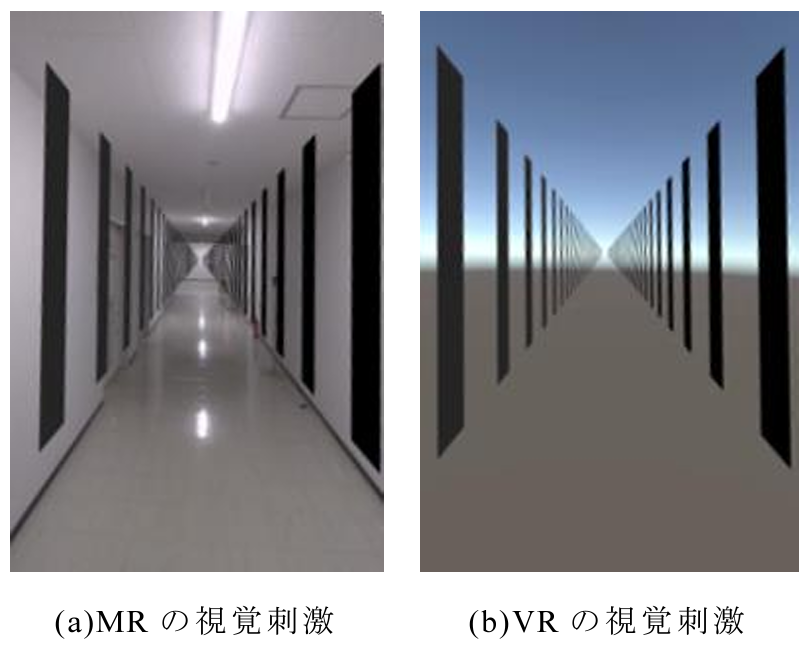
\includegraphics[clip, width=0.8\linewidth]{fig/1.PNG}
    \caption{近藤らの実験で使用された視覚刺激}
    \label{fig:1}
\end{figure}

\subsection{歩行における視覚と運動感覚の整合性}
高幣らは歩行する際に感じる足の接地や筋肉の伸縮などを歩行運動感覚と定義し,
HMDで被験者に対して\figref{fig:2}のような一定速度で空間内を前進する映像を提示し,この提示した速度を視覚速度を定義した.
これらの歩行運動感覚と視覚速度を入出力とし,
自己移動速度のそれぞれの感覚における速度知覚特性とその関係について調べた\cite{takahei}.
その結果,視覚で知覚される移動速度は常に歩行運動感覚で知覚される速度よりも遅く知覚されることがわかった.
\begin{figure}[h]
    \centering
    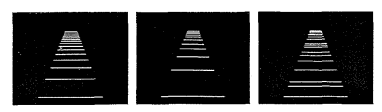
\includegraphics[clip, width=0.9\linewidth]{fig/2.PNG}
    \caption{高幣らの実験でHMDに提示される映像}
    \label{fig:2}
\end{figure}


\section{歩行誘導に関する事例}
路面や標識に印字された記号や文字,警備員による音声案内などの意味を解釈して行動に移させる情報提示を用いず,
意味解釈を必要とせずに歩行者を誘導可能な手法について数多く研究されている.
これらの手法では提示の意味について解釈する過程を必要とせず,
対象者のリソースを消費しないナビゲーション手法として注目されている.
これまでに提案されている手法には,視覚以外の刺激を利用したものと,
本研究と同様に視覚を利用したものがある.

\subsection{視覚以外を使用した歩行誘導方法}
Kojimaらは耳が引っ張ることで歩行ナビゲーションを行う手法であるPull-Naviを提案した\cite{kojima}.
Pull-Naviの概要を\figref{fig:6}に示す.
実験した結果,右左の耳を右左に引っ張ると,被験者はどうしても右,に動きたくなることを確認した.
また,両耳を前方に引っ張ると速く,後方に引っ張ると被験者は遅く歩きたくなったという結果を確認した.
しかし,この手法では耳を引っ張ることで身体に触覚刺激を与えているため,被験者を不快に感じさせる可能性がある.
\begin{figure}[H]
    \centering
    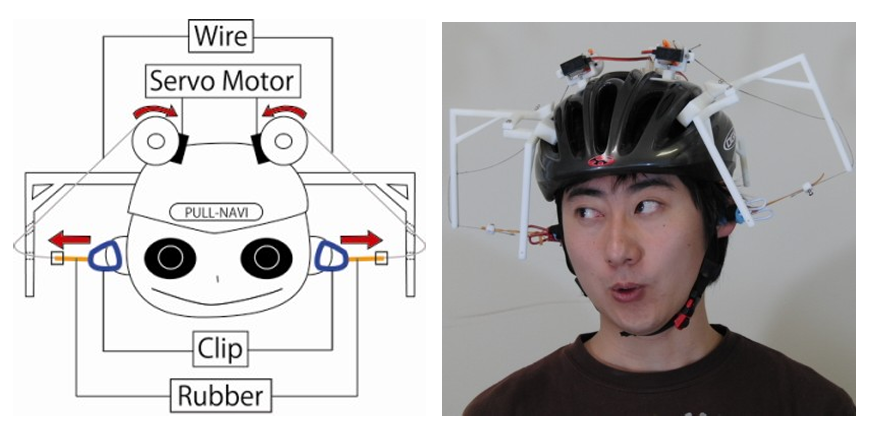
\includegraphics[clip, width=0.8\linewidth]{fig/6.PNG}
    \caption{Pull-Naviの概要図}
    \label{fig:6}
\end{figure}



Freyらは靴の底を傾けて体勢を変化させることで歩行誘導を行う手法を提案した\cite{Frey}.
このシステムでは,靴底に仮想の拡張地形(\figref{fig:10})に変換された道を歩くことになる.
しかし,この手法では靴が傾くことによって足元が不安定になるため,転倒の危険性がある.
\begin{figure}[H]
    \centering
    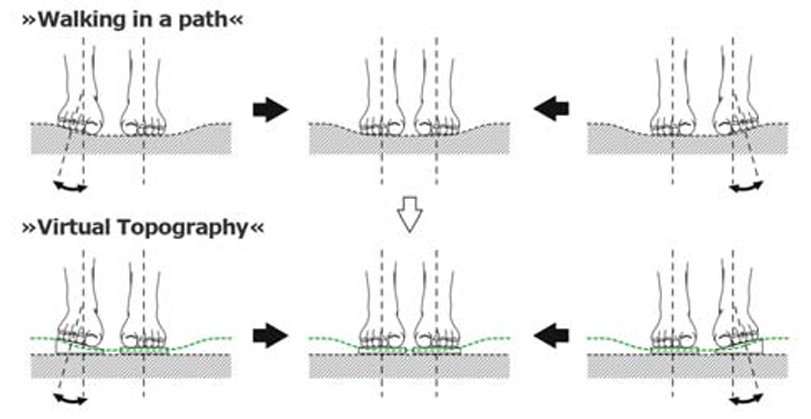
\includegraphics[clip, width=0.8\linewidth]{fig/10.PNG}
    \caption{拡張地形について}
    \label{fig:10}
\end{figure}


\section{視覚刺激を用いた歩行速度制御}
人は五感によって得られる情報のうち,視覚によるものは87\%を占めており,人の行動に大きな影響を及ぼすことが知られている\cite{syomei}.
このことから,視覚刺激は歩行速度制御に適しており,以下のような研究が行われている.
\subsection{プロジェクションマッピングを用いた歩行速度制御}
上田らはプロジェクションマッピングを用いて床にベクション効果を伴う映像\figref{fig:4}を投影し,
被験者に対し,身体的な負担をかけず,無意識に歩行速度を制御できるかを調べた\cite{ueda}.実験環境を\figref{fig:3}に示す.
その結果,プロジェクションマッピングを用いたベクション効果を伴う映像は歩行速度に変化をもたらすことがわかった.
しかし,課題として暗所を歩行する際の安全性の低さが挙げられた.
\begin{figure}[H]
    \centering
    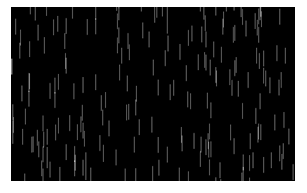
\includegraphics[clip, width=0.6\linewidth]{fig/4.PNG}
    \caption{ベクション効果を伴う映像}
    \label{fig:4}
\end{figure}
\begin{figure}[H]
    \centering
    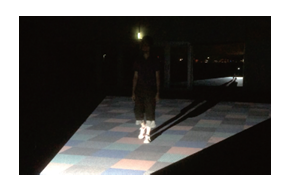
\includegraphics[clip, width=0.6\linewidth]{fig/3.PNG}
    \caption{プロジェクションマッピングにより足元に映像を提示されている被験者}
    \label{fig:3}
\end{figure}





\subsection{周辺視野への刺激提示による速度感増強}
岡野らは周辺視野に対して適切なオプティカルフロー(OF)を提示することによって,
自己運動感覚の中の速度感覚を増強できるかを調べた\cite{okano}.
実験で使用した周辺視ディスプレイを\figref{fig:oka}に示す.
結果として,歩行時の速度感覚が増強されるという効果はあると確認された.
しかし,視野下部に対する刺激と視野側面に対する刺激に関する問題が残っている.
\begin{figure}[H]
    \centering
    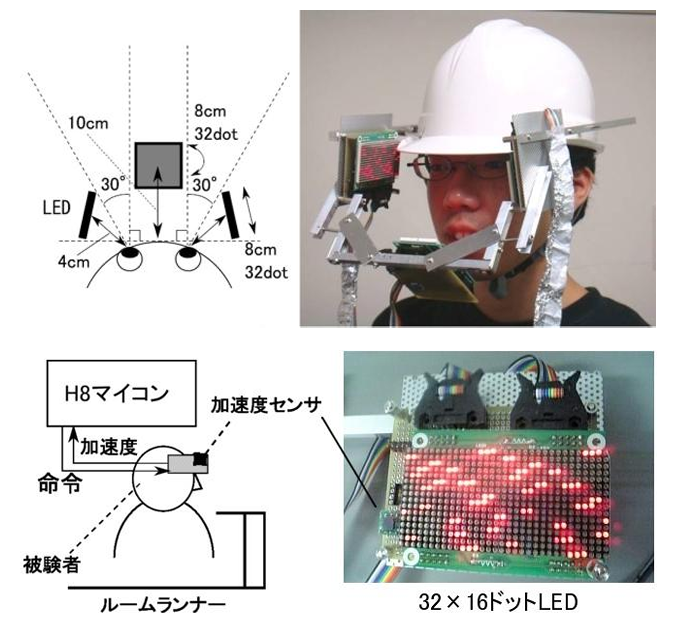
\includegraphics[clip, width=0.7\linewidth]{fig/9.PNG}
    \caption{周辺視野にオプティカルフローを提示するシステム}
    \label{fig:oka}
\end{figure}



\subsection{視覚刺激と身体動揺を利用した歩行誘導}
オプティカルフローは自分の移動の方向と速度を判断する重要な手掛かりとなっている\cite{opu}.
Anoukらはオプティカルフローの速度の変化に応じて被験者が歩行速度を調節できるかをVR空間を使用して調べた\cite{Anouk}.
\figref{fig:9}に実験で用いたVR空間を示す.
結果として知覚するOFの速度が遅いと歩行速度は速く,
逆にOFの速度が速いと歩行速度は遅くなる傾向にあると分かった.
\begin{figure}[H]
    \centering
    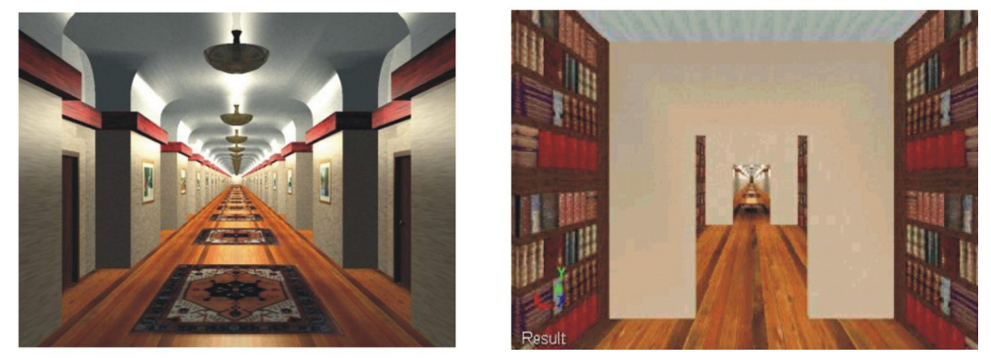
\includegraphics[clip, width=0.9\linewidth]{fig/12.PNG}
    \caption{オプティカルフローを提示するVRシステム}
    \label{fig:9}
\end{figure}


\section{VRを用いた歩行速度制御}
谷崎らは実空間を歩行中の被験者にヘッドマウントディスプレイを通してオプティカルフローの速度と中心視野を変化させたバーチャル空間\figref{fig:5}を提示し,
被験者の歩行速度の変化を調べた\cite{tanizaki}.
その結果,オプティカルフローの速度と被験者の歩行速度の間に負の相関があると示唆された.

\begin{figure}[H]
    \centering
    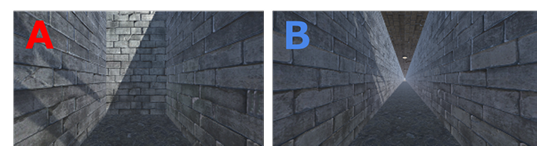
\includegraphics[clip, width=1.0\linewidth]{fig/5.PNG}
    \caption{実験で使用されたバーチャル空間}
    \label{fig:5}
\end{figure}

谷崎らは.VR空間内で並走するバーチャルアバタの並進の
速度,形態,歩行運動の動きの3つの要因に対して自然歩行時の歩行速度が
変化するかを調べた\cite{heiso}.
並走するバーチャルアバタの存在するバーチャル空間を\figref{fig:15}に示す.
その結果,並走するアバタの形態と運動による歩行速度変調が確認された.
しかし,長距離や長時間,実験環境外の環境でのシステムの有用性は確認できていない.
\begin{figure}[H]
    \centering
    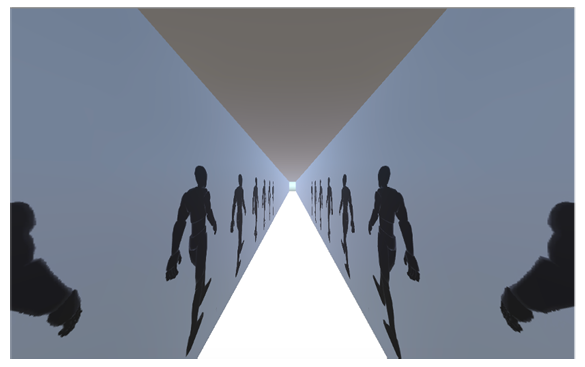
\includegraphics[clip, width=0.9\linewidth]{fig/15.PNG}
    \caption{実験で使用された並走するバーチャルアバタの存在するバーチャル空間}
    \label{fig:15}
\end{figure}


これらの手法はVRに基づいており,現実空間の歩行速度誘導に利用するのことは難しい.

\section{ARを用いた歩行速度制御}
櫻木らはARグラスを通して見える床面上に「動く歩道」のテクスチャをアニメーション提示し,
その際の被験者の歩行運動を観察した\cite{sakura}.
この手法はARに基づいており,現実空間の歩行速度誘導への適合性が高いものの,
著者らが期待した誘導効果は確認できなかった.
その理由として,ARで提示したテクスチャの見た目(\figref{fig:8})が現実の床面の見た目と差があること,
歩行の際にテクスチャの隙間から床面が見えてしまい,被験者からみた現実感(被験者から見える空間の整合性)が低下したことの影響を挙げている.

\begin{figure}[H]
    \centering
    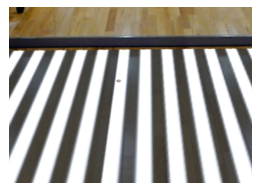
\includegraphics[clip, width=0.9\linewidth]{fig/8.PNG}
    \caption{実験で使用されたテクスチャ}
    \label{fig:8}
\end{figure}
\section{本稿の位置付け}
本研究では個々の歩行者に対し,確実な指示伝達を行うのにARが適していると考える.
また,ARを用いた行動制御方法では実際の歩行面に近いテクスチャーをトラベレーターのようにアニメーションすることで
拡張現実的なアプローチでも誘導効果が得られ,被験者の動きをより制御できると考える\cite{moto}.
本稿では芝生道にて,芝生を模したバーチャル床を表示した場合と芝生を模していないバーチャル床を表示した場合
を比べて被験者の歩行速度制御に有位性が出るか否かの調査する.		% 第2章 関連技術
\chapter{TravelatAR : 地表面近似テクスチャーのアニメーション重畳表示による歩行速度制御システム}
本システムではユーザの視界に映る床へ現実の床を模したバーチャル床が被験者に対して前から流足元へ流れてくるようなアニメーション重畳表示する.
これにより,被験者の自己運動感覚を操作し意味解釈を必要としない歩行速度操作を行う.
\section{システム概要}
\figref{fig:gaiyo}に本システムの概要を示す.
本システムでは被験者にARグラスを装着してもらう.
これにより,仮想空間に存在する現実の床を模したバーチャル床をユーザの視界の床へアニメーション重畳表示する.
\begin{figure}[h]
    \centering
    \fbox{
        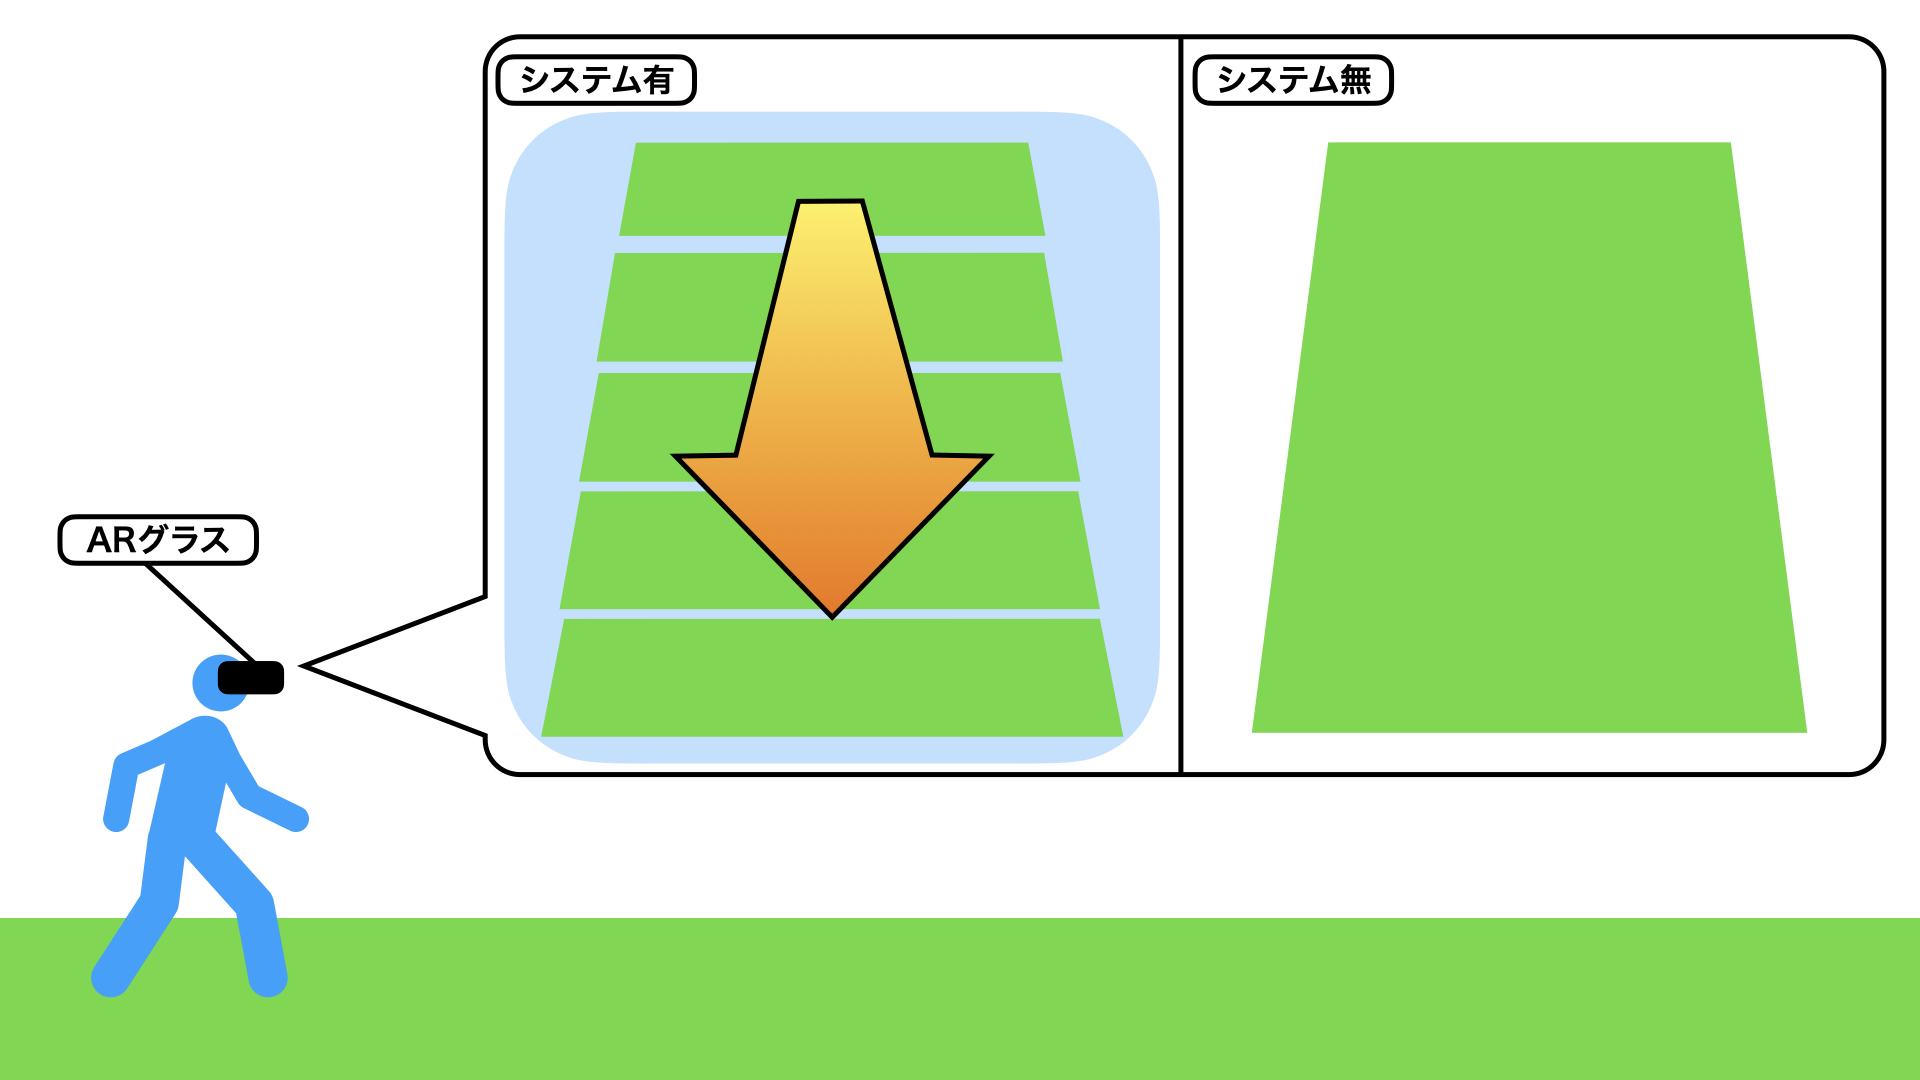
\includegraphics[width=0.8\linewidth]{fig/gaiyo.001.jpeg}
    }
    \caption{システム概要図}
    \label{fig:gaiyo}
\end{figure}

\begin{figure}[ht]
    \centering
    \fbox{
        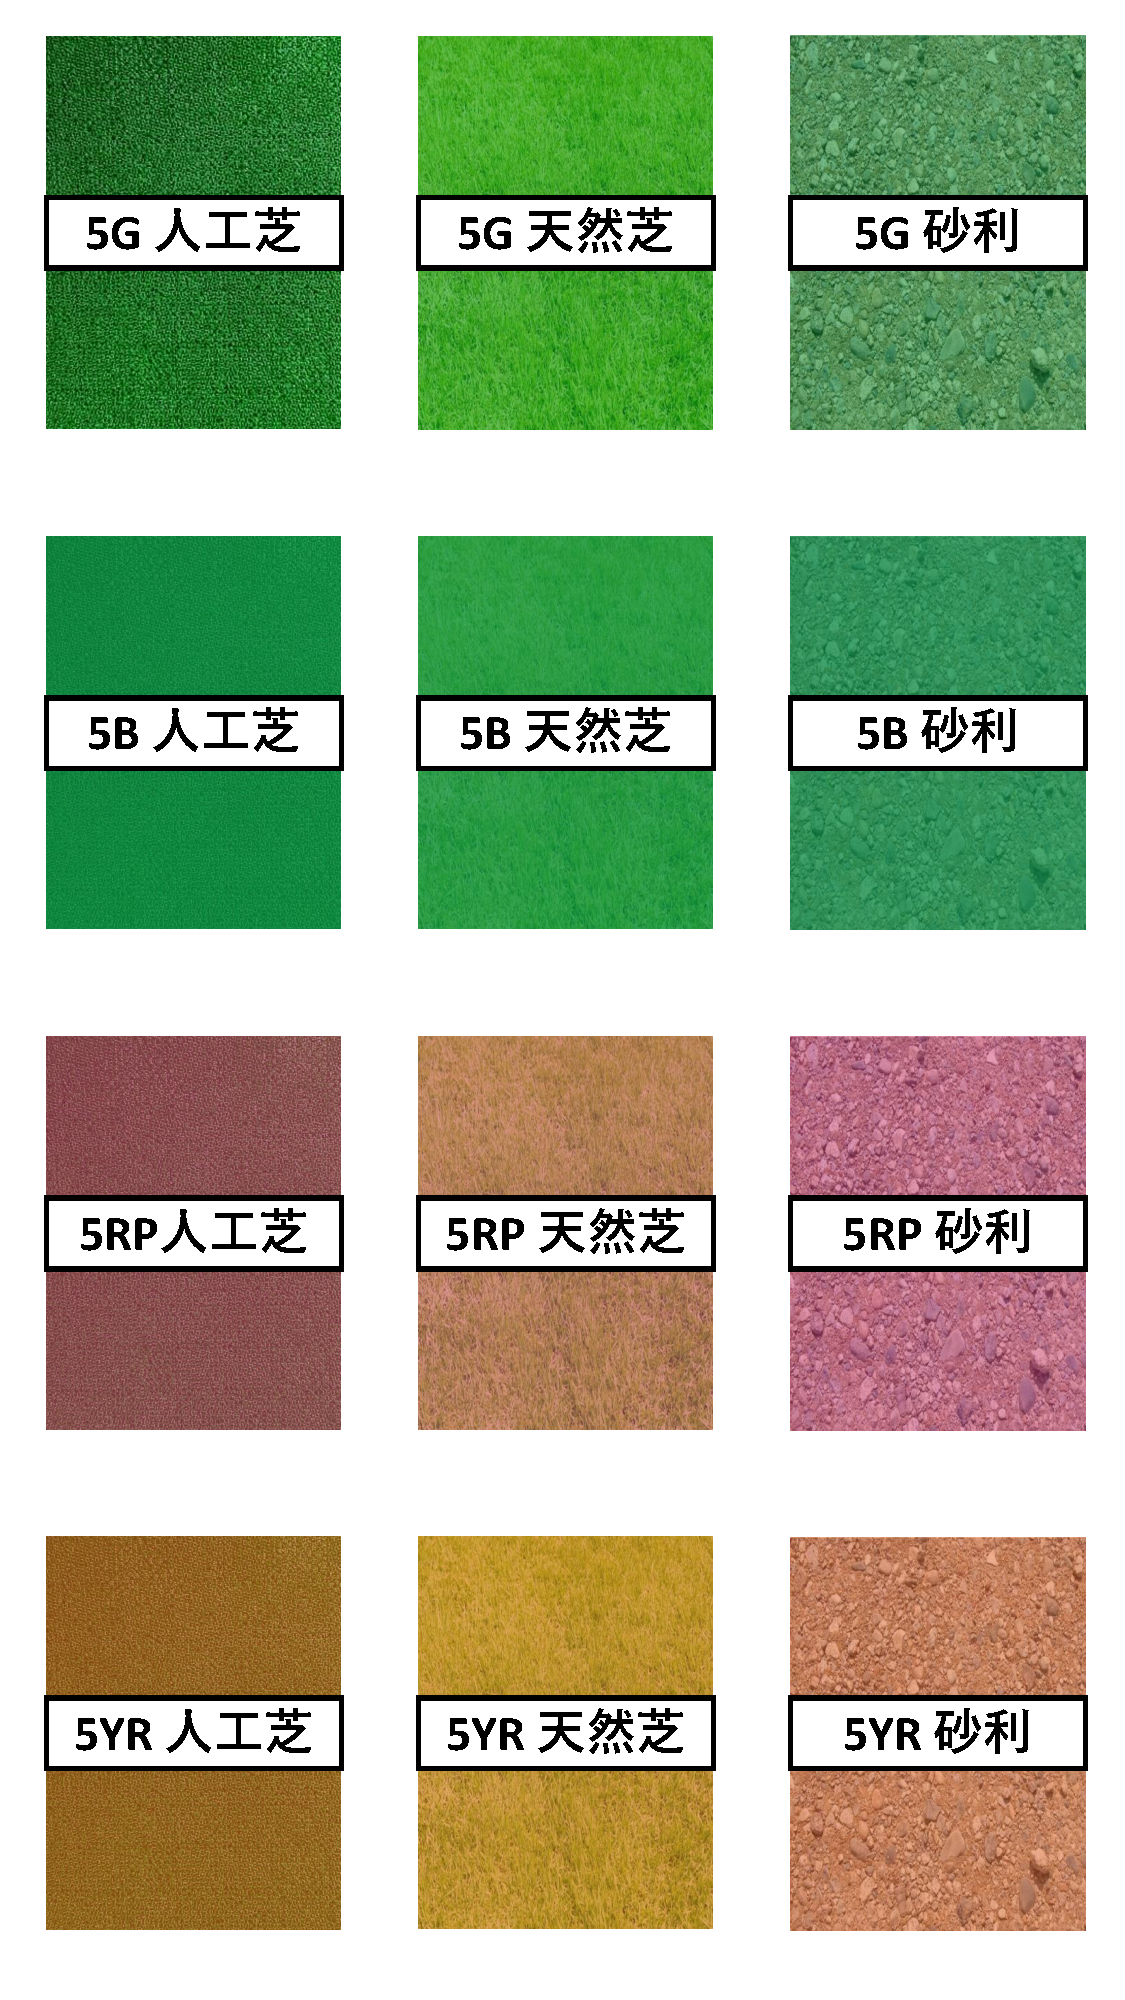
\includegraphics[width=0.7\linewidth]{fig/マテリアル.pdf}
    }
    \caption{リアルテクスチャ(5G人工芝)・Nonリアルテクスチャ一覧}
    \label{fig:Nrial}
\end{figure}


\section{リアルテクスチャ}
ユーザが歩く道の地表面に近似したテクスチャを作成する.
本システムでは,これらのテクスチャをバーチャル床にアタッチし被験者の視界の床へアニメーション重畳表示を行う.
本実験では人工芝の道を歩くことを想定したリアルテクスチャ作成した.
また,リアルテクスチャの比較対象となる地表面に近似していないNonリアルテクスチャを複数作成した.

\section{Nonリアルテクスチャ}
\figref{fig:Nrial}にリアルテクスチャとNonリアルテクスチャの一覧を示す.
リアルテクスチャは,色と模様を地表面に近似させ,作成している.
色は,人工芝と同じ色である5G,色相環で5Gの反対に位置する5RP,それらの中間に位置する5YR,5Bを使用した\cite{color}.
模様は,人工芝に近似させたもの,人工芝に近いものとして天然芝,そして,人工芝に近似させない物として砂利を用意した.
今回Nonリアルテクスチャはリアルテクスチャを含む12通りで作成した.


\section{バーチャル床}
バーチャル床は仮想空間内に存在する仮想オブジェクトである.
このオブジェクトに上記で説明したリアルテクスチャかNonリアルテクスチャをアタッチし
ARグラスを通してユーザへ次々と提示する.
また,このオブジェクトはシステムの負荷を下げるため,ユーザが踏んだ際に消える設定となっている.
ユーザへ提示される際,ユーザの視界の床に前から迫ってくるなどのアニメーション重畳表示される.

\section{実装}
本システムはunityを用いて作成を行った\cite{unity}.
今回の実験では歩く道が固定であったため,バーチャル床を発生させる位置をユーザの正面20m先に固定した.
発生するバーチャル床はユーザの頭の位置から1.6m下の位置を移動する.この1.6mは被験者たちの身長から調整を行った.	% 第3章 提案
\chapter{評価}
著者らはTravelatARを用いて評価実験を行った.
\section{実験環境}
\figref{fig:env}に実験時の環境を\figref{fig:siten},\figref{fig:nonsiten}は被験者の視界を示す.
被験者は20代の男性6名である.
本システムでは道芝\cite{siba}にて,リアルテクスチャをアタッチしたバーチャル床をアニメーション重畳表示した場合と
Nonリアルテクスチャをアタッチしたバーチャル床をアニメーション重畳表示した場合
を比べてユーザの歩行速度制御に有位性が出るか否か調査する.
道芝の長さは20メートルとなっている.
今回使用するシステムでバーチャル床は,\figref{fig:maekara}のよう,ユーザに向かってくるよう動く.
被験者は頭にARグラスのHoloLens2を,体にはiPhone11 proを揺れないよう固定して装着してもらう\cite{holo}\cite{ipon}.
\begin{figure}[H]
    \centering
    \fbox{
        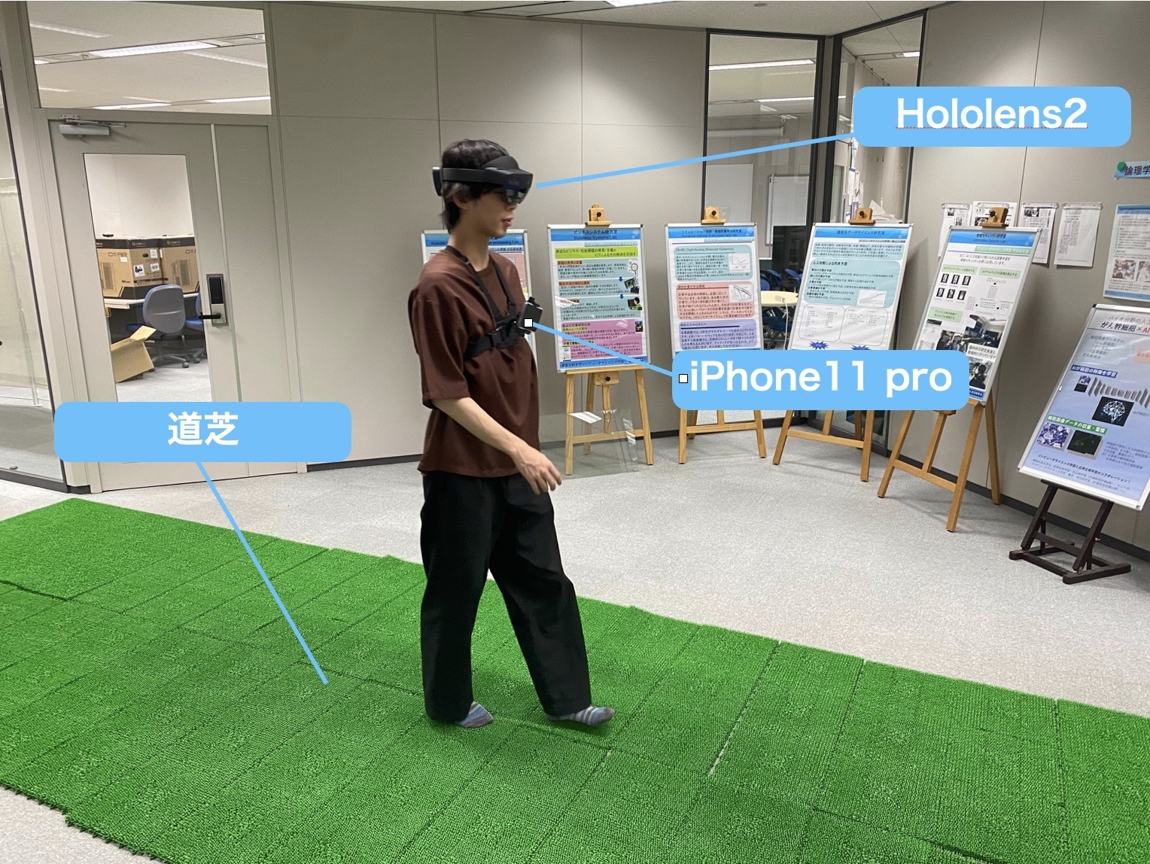
\includegraphics[keepaspectratio, width=0.6\linewidth]{fig/enviroment.png}
    }
    \caption{実験環境}
    \label{fig:env}
\end{figure}
\begin{figure}[H]
    \centering
    \fbox{
        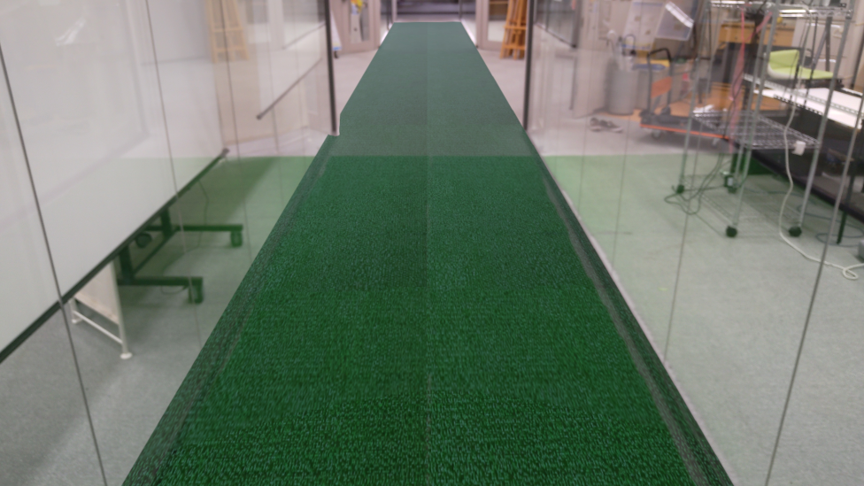
\includegraphics[width=0.8\linewidth]{fig/siten.png}
    }
    \caption{ユーザの視界(リアルテクスチャ適用)}
    \label{fig:siten}
\end{figure}
\begin{figure}[H]
    \centering
    \fbox{
        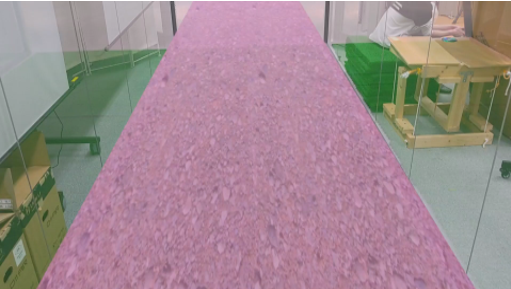
\includegraphics[width=0.8\linewidth]{fig/nonreal.PNG}
    }
    \caption{ユーザの視界(Nonリアルテクスチャ適用(5RP砂利))}
    \label{fig:nonsiten}
\end{figure}

\begin{figure}[H]
    \centering
    \fbox{
        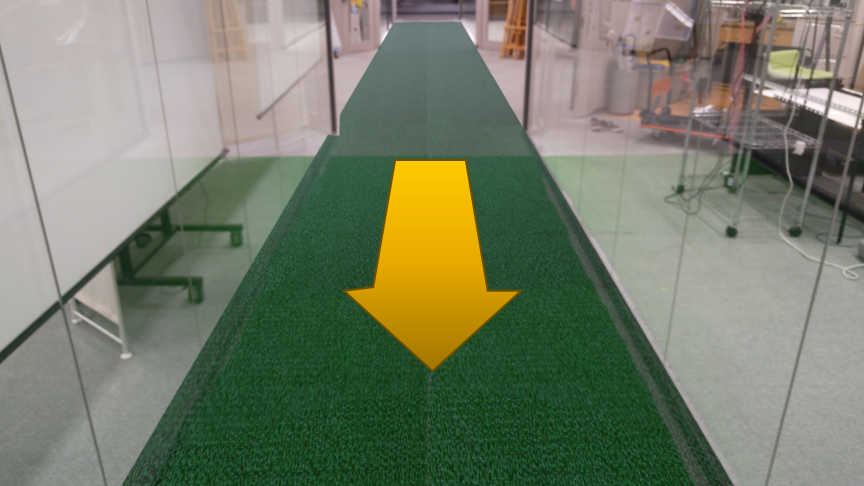
\includegraphics[width=0.8\linewidth]{fig/11.png}
    }
    \caption{本実験でのバーチャル床の動き}
    \label{fig:maekara}
\end{figure}

\section{実験手順}
実験手順を以下に示す.
\begin{enumerate}
    \item スタート地点に直立してもらった
    \item 被験者の装着しているiPhone11 proのセンサーのスイッチをオンにした
    \item 指定距離歩いてもらう
    \item 歩き終わった位置で直立してもらう
    \item センサーのスイッチをオフにする
\end{enumerate}
上記の手順を6回同じシステムで繰り返してもらい,それを1セットとした.
また,1セット終わるたびアンケートに回答してもらった.
この手順をシステムを使用していない状態のHoloLens2を装着した状態,
12種類の本システムを使用した状態の計13セット行ってもらった.



\section{評価方法}
本稿では定性評価と定量評価を行う.


定性評価では,酔いに関する主観的評価尺度であるThe Simulator Sickness Questionnaire((SSQ))\tabref{tab:SSQ}によるアンケートをとる\cite{ssq}.
その後,リアルテクスチャに関して,実際に床が動いているよう感じたかの他,
歩いている速度が早く感じるか,遅く感じるかといった感覚を速度感と定義して
システム未使用時に比べ,速い速度感を得たかと遅い速度感を得たかを
それぞれの1(まったく感じなかった)~5(非常に感じた)までの5段階のリッカート尺度を用いたアンケートを取る.
アンケートの最後には自由記述欄も用意した.
\begin{table}[h]
    \begin{center}
        \caption{The Simulator Sickness Questionnaire} \label{tab:SSQ}
        \begin{tabular}{c|l}\hline\hline
            質問番号 & 質問項目                                             \\\hline
            1        & 一般的な不快感がある                                 \\
            2        & 疲労感がある                                         \\
            3        & 頭痛がする                                           \\
            4        & 眼が疲れている                                       \\
            5        & 眼の焦点がぼける                                     \\
            6        & 唾液が増えている                                     \\
            7        & 発汗している                                         \\
            8        & 吐き気がする                                         \\
            9        & 集中できない                                         \\
            10       & 頭が重い                                             \\
            11       & 眼がかすむ                                           \\
            12       & (眼を開けた状態で)フラッとするようなめまい感がある \\
            13       & (眼を閉じた状態で)フラッとするようなめまい感がある \\
            14       & 自分や周囲が回転するようなめまいがある               \\
            15       & 胃の存在感がある                                     \\
            16       & げっぷが出る                                         \\\hline
        \end{tabular}
    \end{center}
\end{table}


定量評価では被験者の体に装着されたiPhone11 proの加速度センサー
を用いて歩行時間を計測し,評価する.
その際,以下の組み合わせごとに6回の「ゴールまで歩いた時間」の平均値を比べ,リアルテクスチャの有用性を評価した.
\begin{quote}
    \begin{itemize}
        \item システム無し・システム有(リアルテクスチャ)
        \item システム無し・システム有(11種類のNonリアルテクスチャそれぞれ)
    \end{itemize}
\end{quote}







\section{実験結果}

定性評価の結果を以下に示す.
\figref{fig:anke1}にシステム未使用時に比べ,速い速度感を得たか,
\figref{fig:anke2}にシステム未使用時に比べ,遅い速度感を得たか,
\figref{fig:anke3}にバーチャル床は本物の床が動いているように見えたかのアンケート結果を示す.
これらの棒グラフは,左から1(まったく感じなかった)~5(非常に感じた)となっている.
\figref{fig:anke1}から,色は人工芝の反対であり,模様も近似させていない5RP砂利がもっとも速い速度感を被験者に与えたことがわかった.
また,\figref{fig:anke2}からはほとんどのテクスチャが遅い速度感を与えなかったことがわかるが,5G天然だけは被験者によって意見が分かれている.
\figref{fig:anke3}から,リアルテクスチャである5Gは12種類のテクスチャの中で一番本物の床が動いているように見えたという結果を得た.
\begin{figure}[H]
    \centering
    \fbox{
        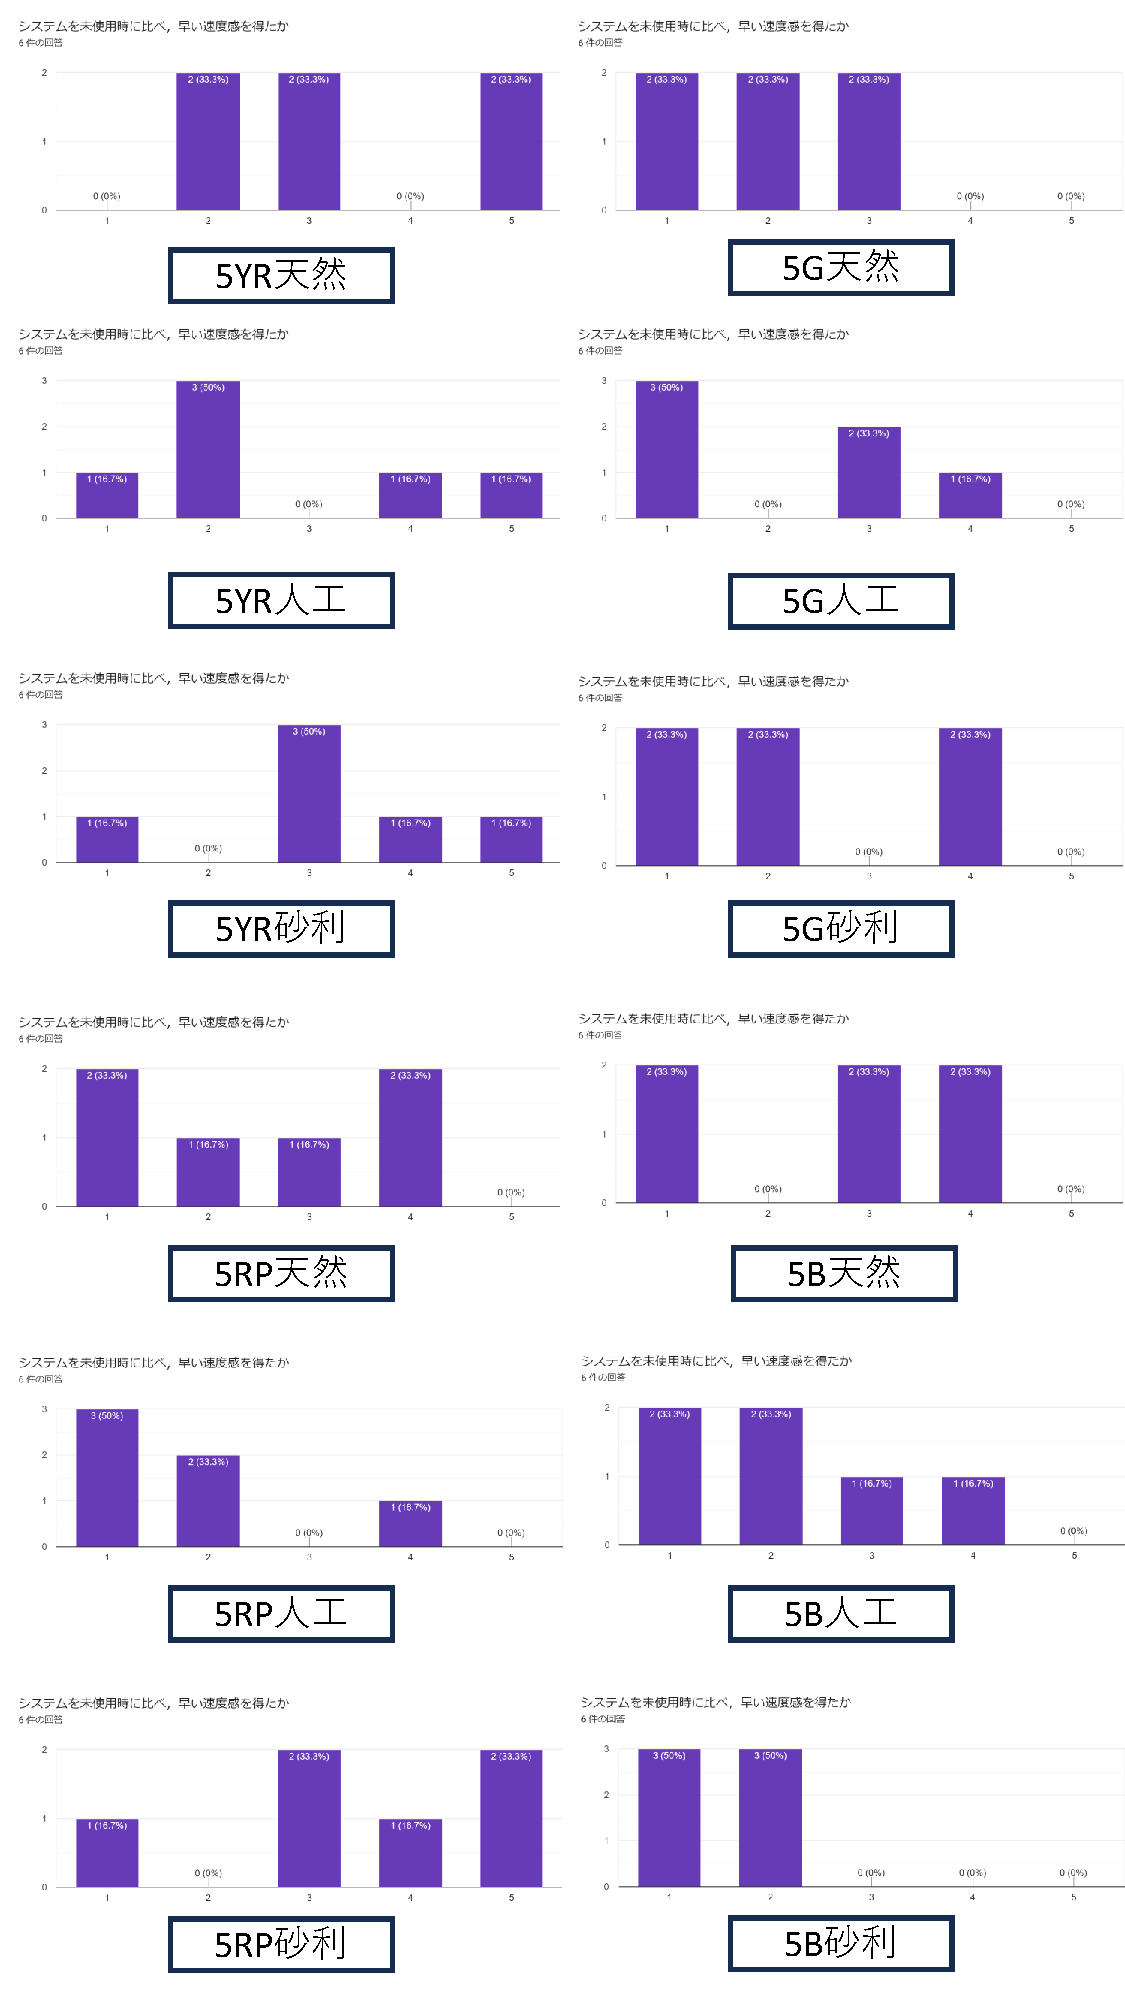
\includegraphics[width=0.7\linewidth]{fig/アンケート結果.pdf}
    }
    \caption{主観的な速度感に関するアンケート結果(上昇)}
    \label{fig:anke1}
\end{figure}

\begin{figure}[H]
    \centering
    \fbox{
        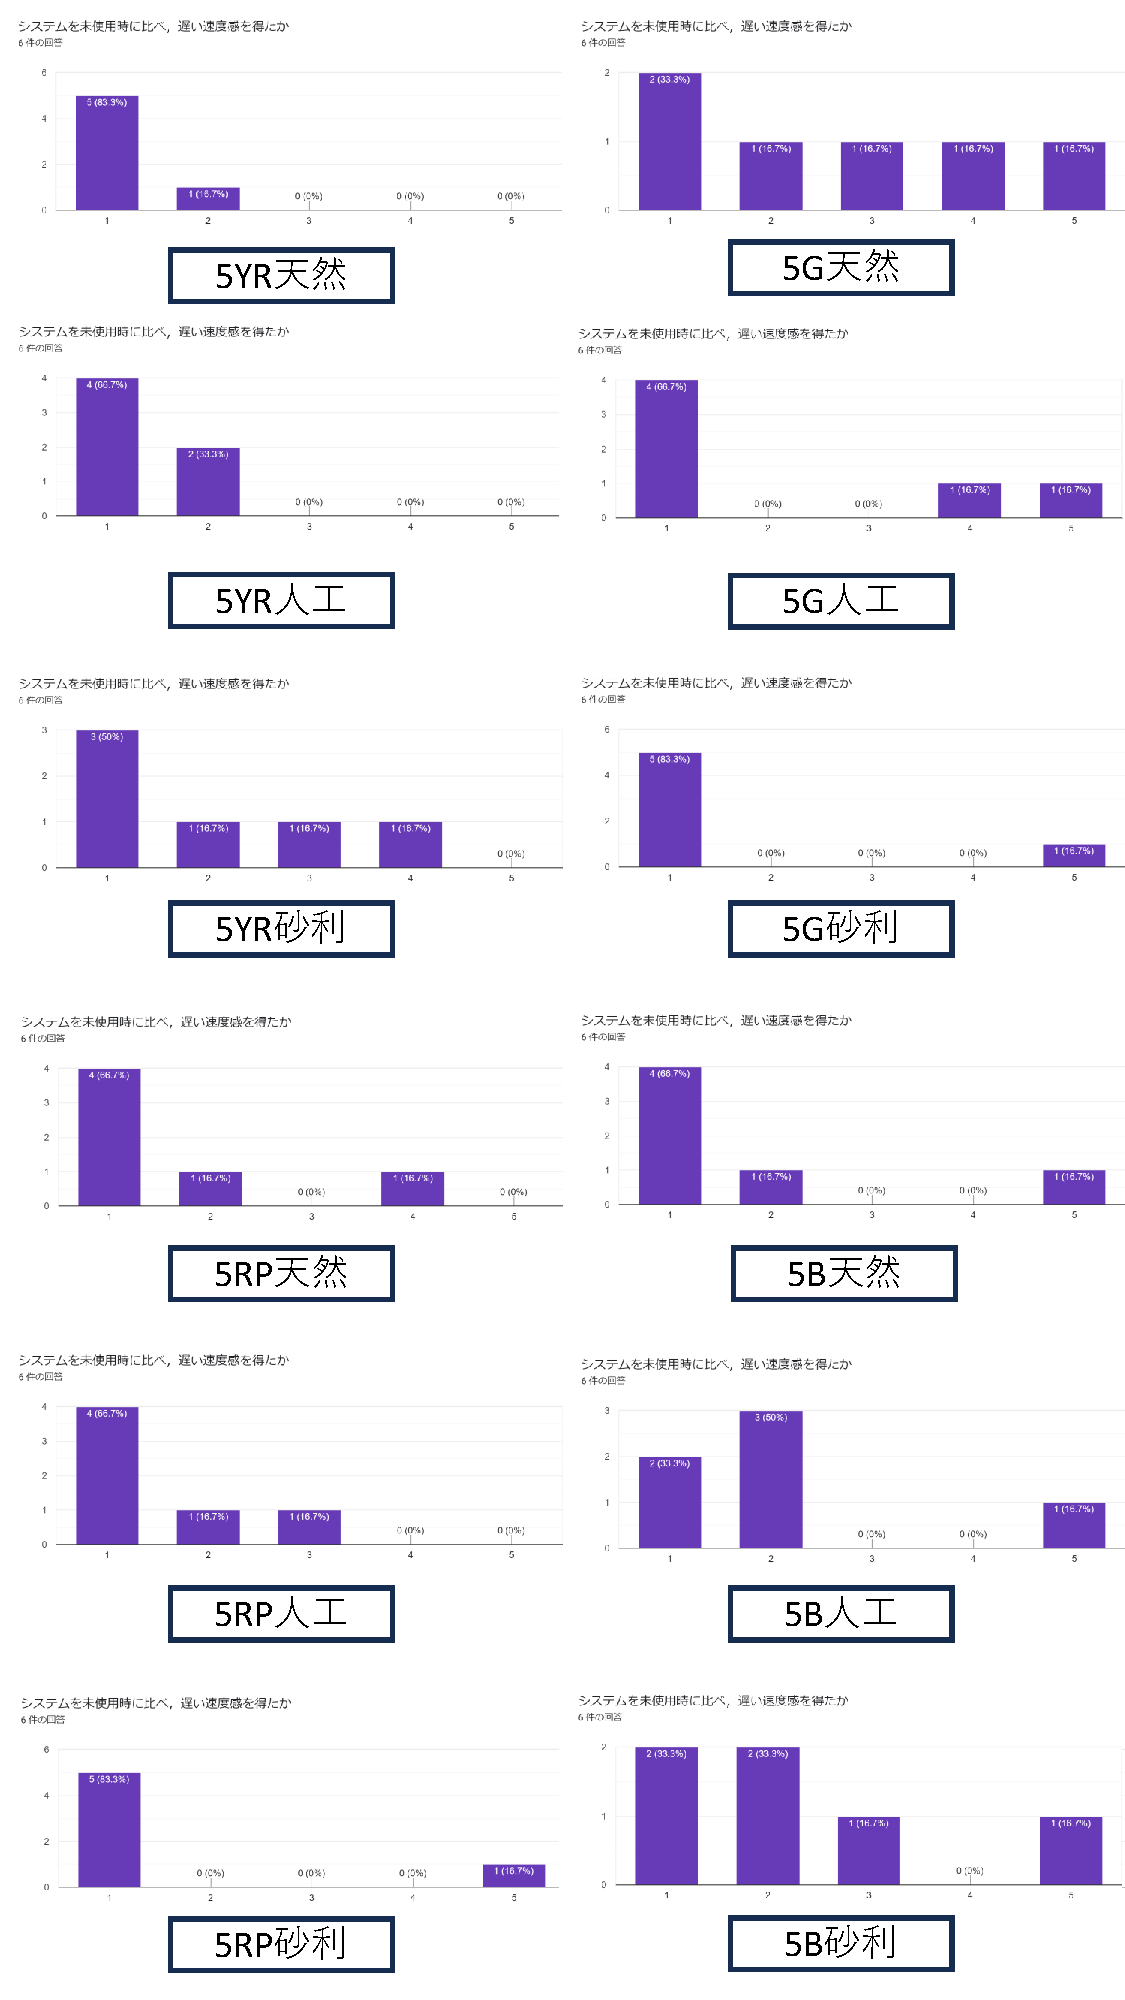
\includegraphics[width=0.7\linewidth]{fig/アンケート結果2.pdf}
    }
    \caption{主観的な速度感に関するアンケート結果(下降)}
    \label{fig:anke2}
\end{figure}

\begin{figure}[H]
    \centering
    \fbox{
        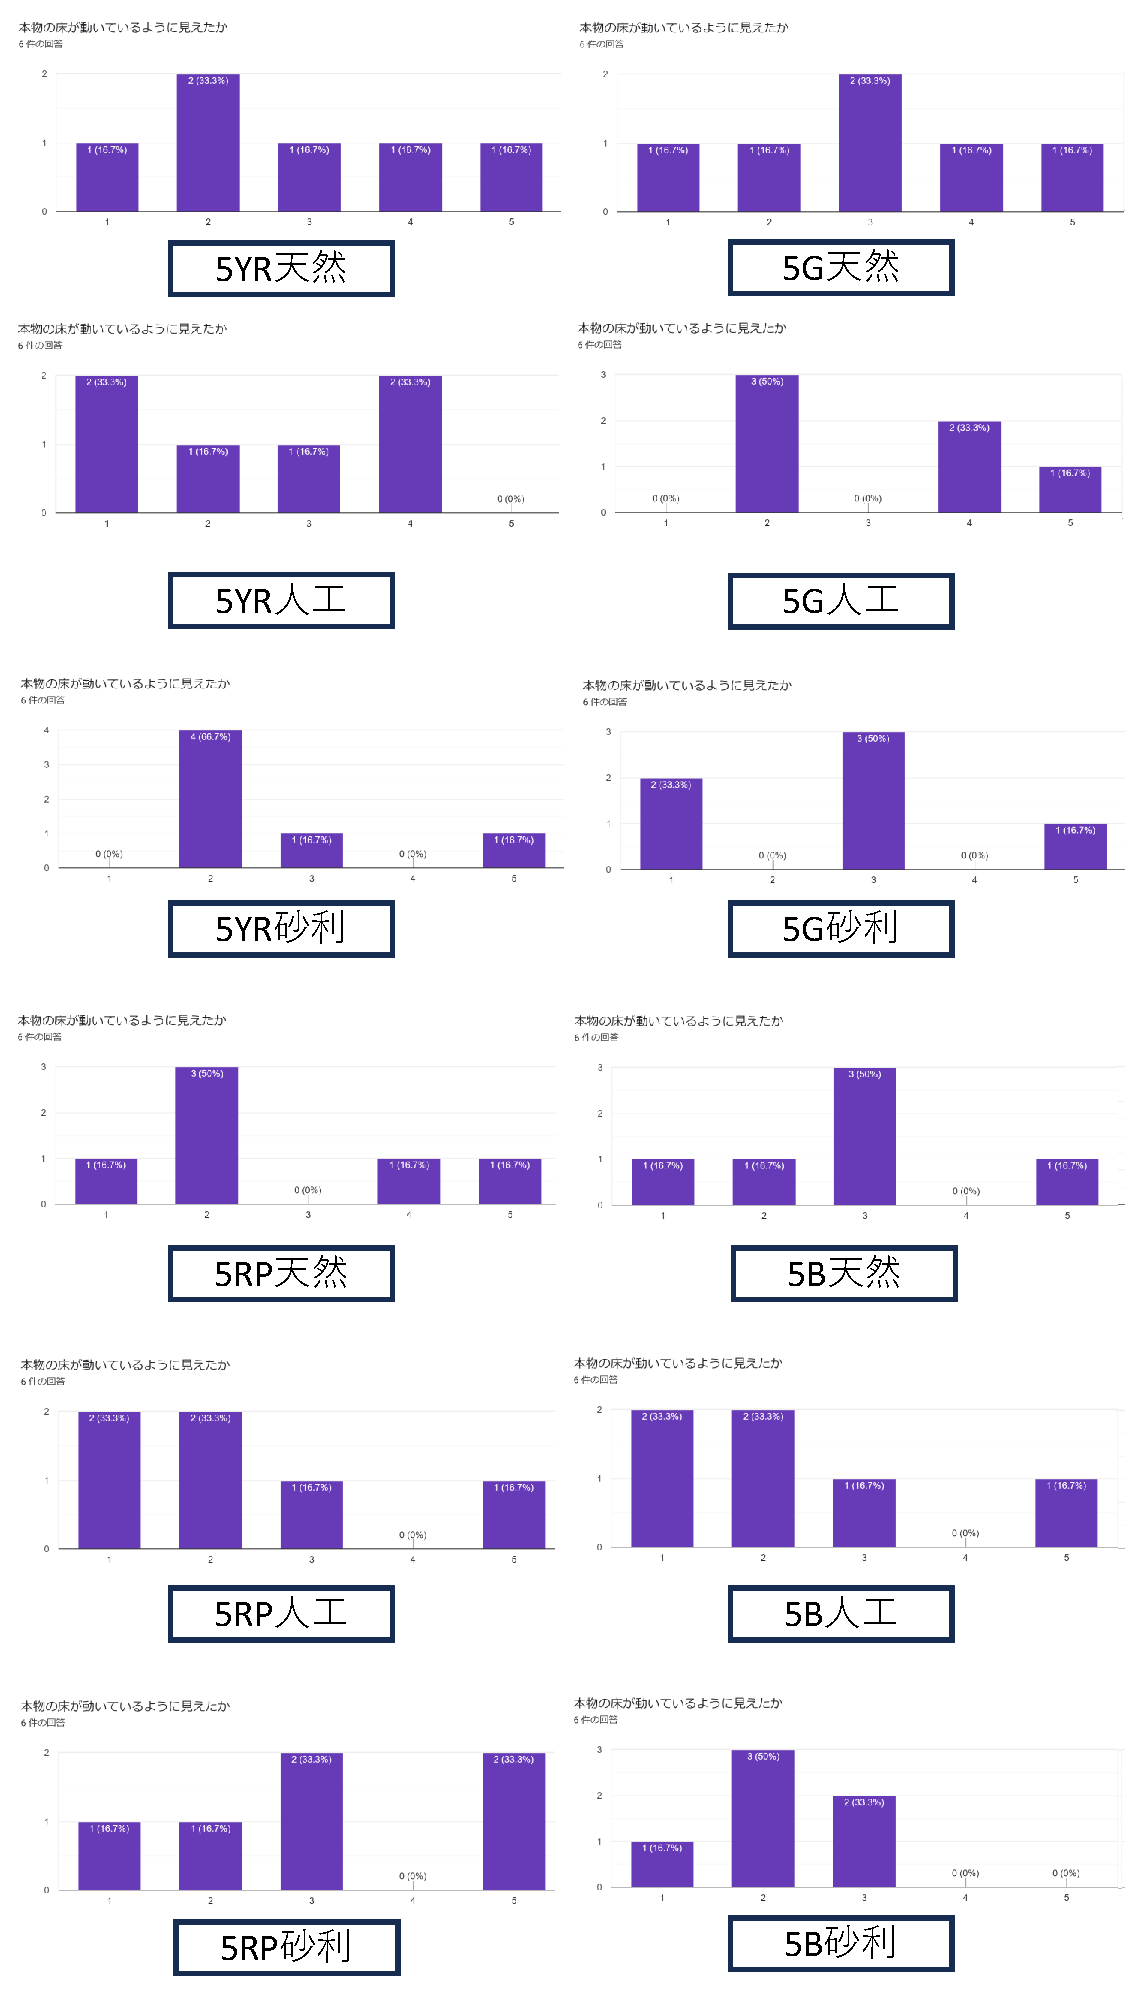
\includegraphics[width=0.7\linewidth]{fig/アンケート結果3.pdf}
    }
    \caption{本物の床が動いているように見えたかのアンケート結果}
    \label{fig:anke3}
\end{figure}




定量評価の結果を以下に示す.
\figref{fig:teiryo}にシステム未使用時とシステム使用時のゴールまでの時間差の一覧を示す.
被験者によって,歩行時間がプラスやマイナスになってしまっている.
また,SSQによる映像酔いの調査結果は上記の評価に対して影響は確認できなかった.
\begin{figure}[H]
    \centering
    \fbox{
        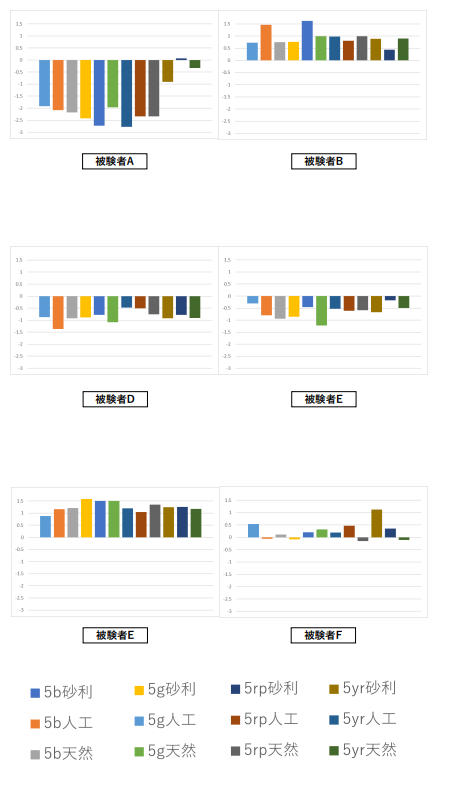
\includegraphics[width=0.7\linewidth]{fig/sokudo.PNG}
    }
    \caption{システム未使用時とシステム使用時のゴールまでの時間差一覧}
    \label{fig:teiryo}
\end{figure}



\section{考察}
定性評価から,今回仮説としてユーザの行動制御ができると考えていたリアルテクスチャは,
現実の床に近似させることは成功したが,
あまり速度感に対する成果ははっきりしなかった.
理由として,「システム未使用時に比べ,速い速度感を得たか」の質問では速度感を得た被験者と得られなかった被験者の数は同数だったことが挙げられる.
このことから,被験者を増やすことでより正確な評価を取る必要があると考える.
コメントでは「目の前で床が消えるので,そこで現実に戻されているような気がする」や
「表示されている床に透明感が強く,実際の床が見え,あまり影響がないように感じた」,「芝が虹色になっている部分がありました」
などの,実験環境の影響によりテクスチャを正確に評価できていない場面もあったため,実験環境を改善する必要があると考えられる.
その他コメントに「速く移動しているようにも感じるし,たくさん移動しているようにも感じた」という意見もあり,
速度感の他に距離感にも影響があると示唆された.

定量評価からは,
どのテクスチャでも有意性を見ることができなかった.
その要因として,実験中の被験者の発言から歩く回数の多さからの疲労や上記のコメントから実験環境に問題があると考えられる.
また,歩行速度が速くなっている被験者と遅くなっている被験者の数はほぼ同じことから,より被験者を増やす必要もあると考える.

また,今回の実験ではバーチャル床が前から被験者に迫ってくる動きを実装したが,後ろから被験者を追い越すように動かすなど,
他のバーチャル床の動きを試すことで別の効果が出るのではないかと考察する.
	% 第4章 実装
\chapter{追加実験}

第4章での考察を踏まえTravelatARの改良,実験環境の改善をし,追加実験を行った.

\section{TravelatARの改良}
第4章での考察を踏まえて行ったTravelatARの改良について示す.
バーチャル床の使用を以下の通り変更した.
「目の前で床が消えるので,そこで現実に戻されているような気がする」
とあったことから,バーチャル床を消すタイミングが速いことを確認できたため,
ユーザが踏んだ際では無く通り過ぎた際に消えるよう設定の変更した.
また,バーチャル床の動かし方は,従来の動き方の「前からユーザに向かってくる」と新しく「後ろからユーザを追い越す」\figref{fig:14}
の2つの動かし方をする.
\begin{figure}[H]
    \centering
    \fbox{
        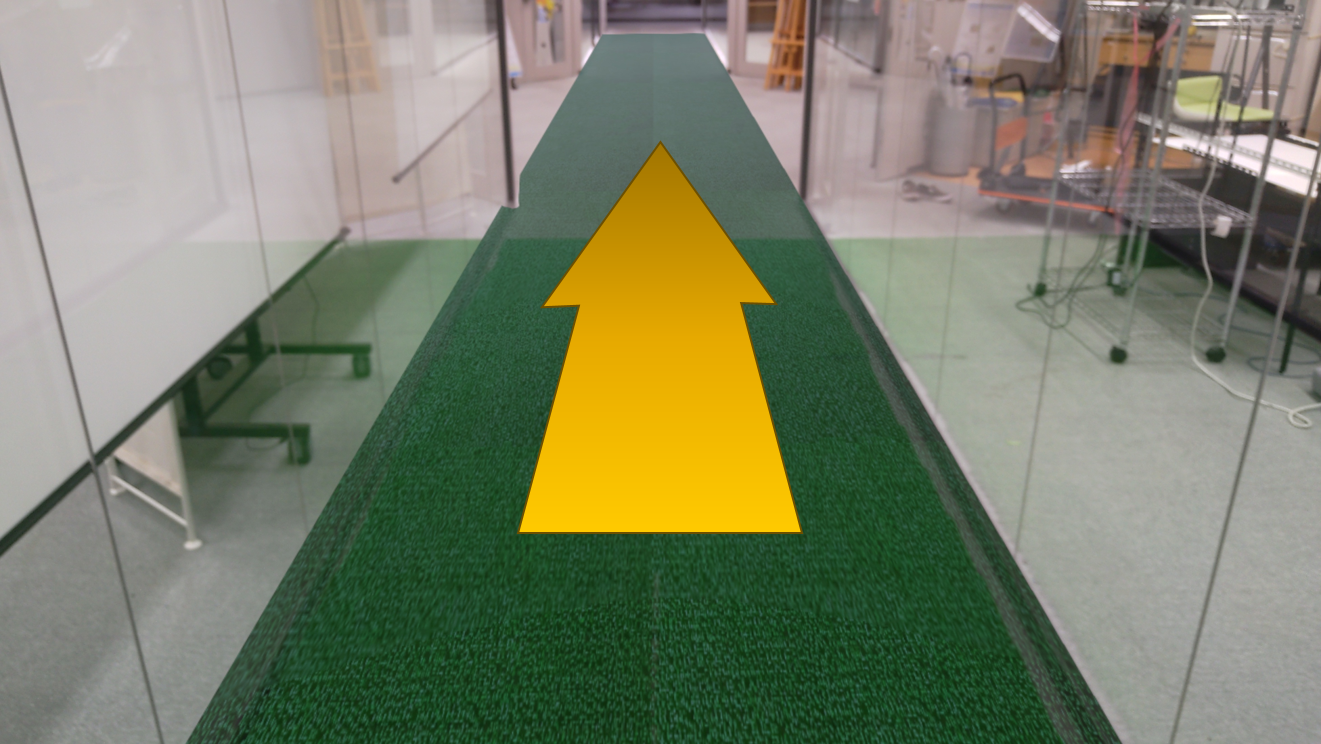
\includegraphics[width=0.7\linewidth]{fig/14.png}
    }
    \caption{後ろからユーザを追い越すバーチャル床のイメージ}
    \label{fig:14}
\end{figure}

\section{実験環境}
被験者は20代の男性7名である.
実験環境を\figref{fig:addgaiyo}に示す.
被験者に付けていたiPhone11 proは付けず,
歩いてもらうコース上には通過センサーとArduino\figref{fig:13.1}を\figref{fig:13}のよう設置する\cite{tuka}.
これにより,正確なユーザの歩行速度を測った.
また,\figref{fig:siten2}コースの照明を消すことで「表示されている床に透明感が強く,実際の床が見え,あまり影響がないように感じた」
「芝が虹色になっている部分がありました」といった照明によるテクスチャの評価への影響を軽減させた.

\begin{figure}[H]
    \centering
    \fbox{
        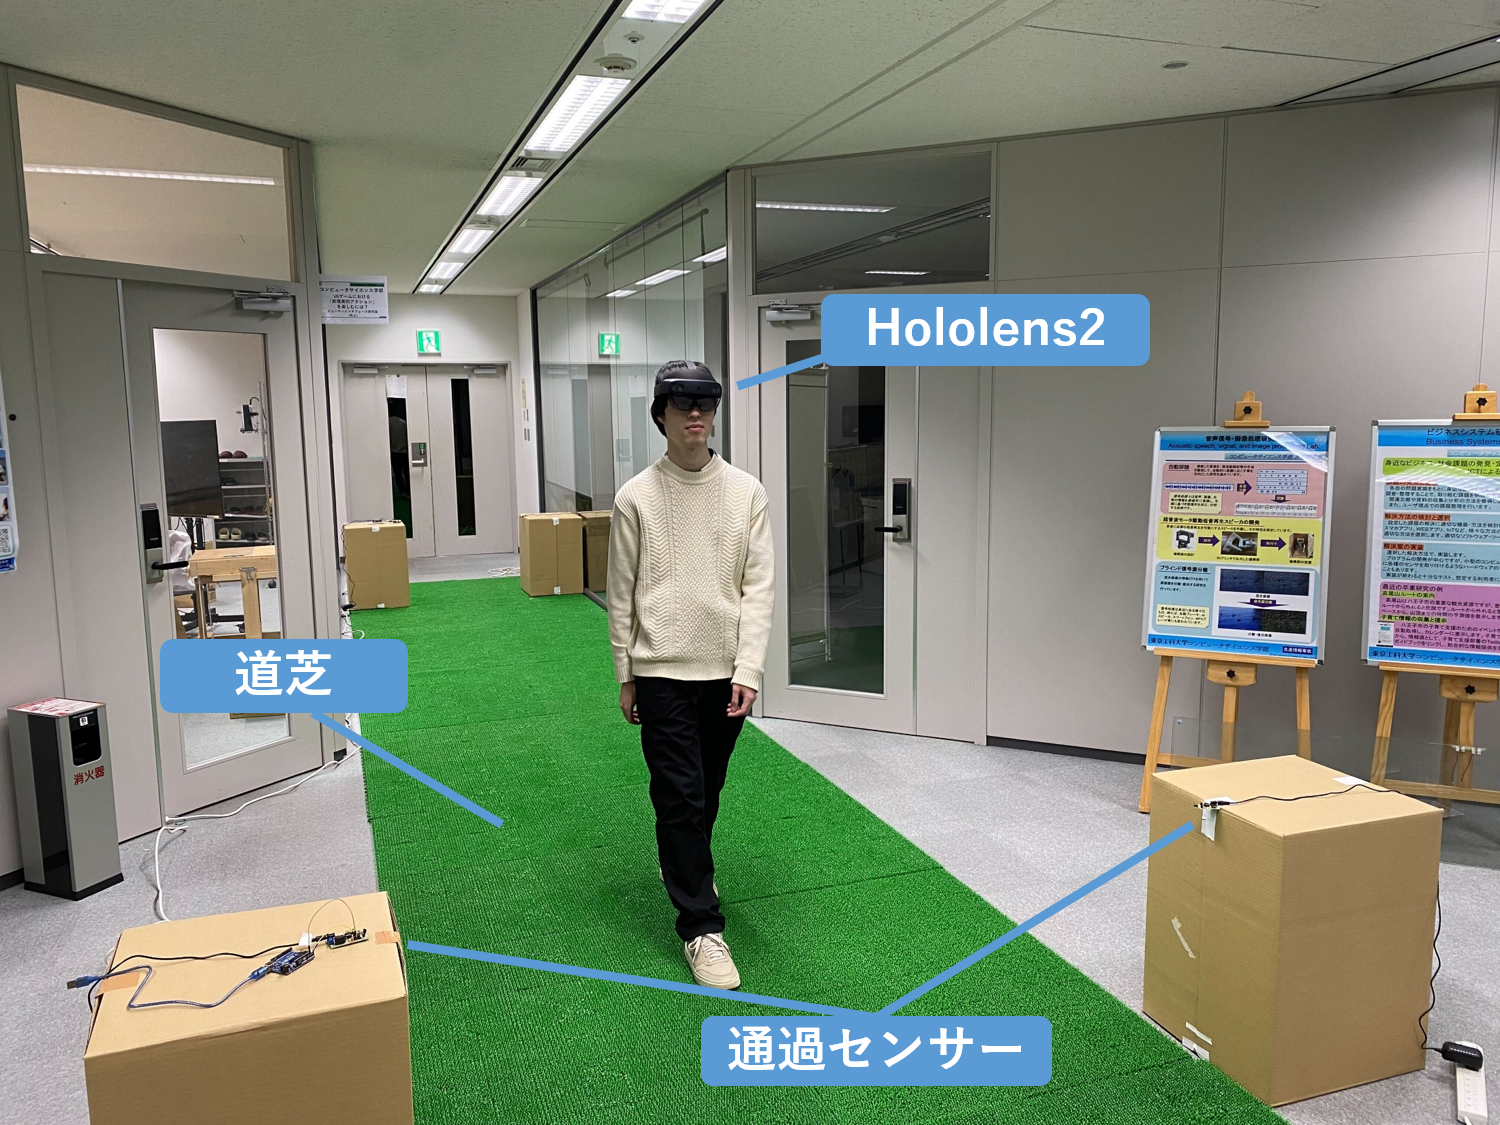
\includegraphics[width=0.7\linewidth]{fig/gaiyo.png}
    }
    \caption{追加実験での実験環境}
    \label{fig:addgaiyo}
\end{figure}
\begin{figure}[H]
    \centering
    \fbox{
        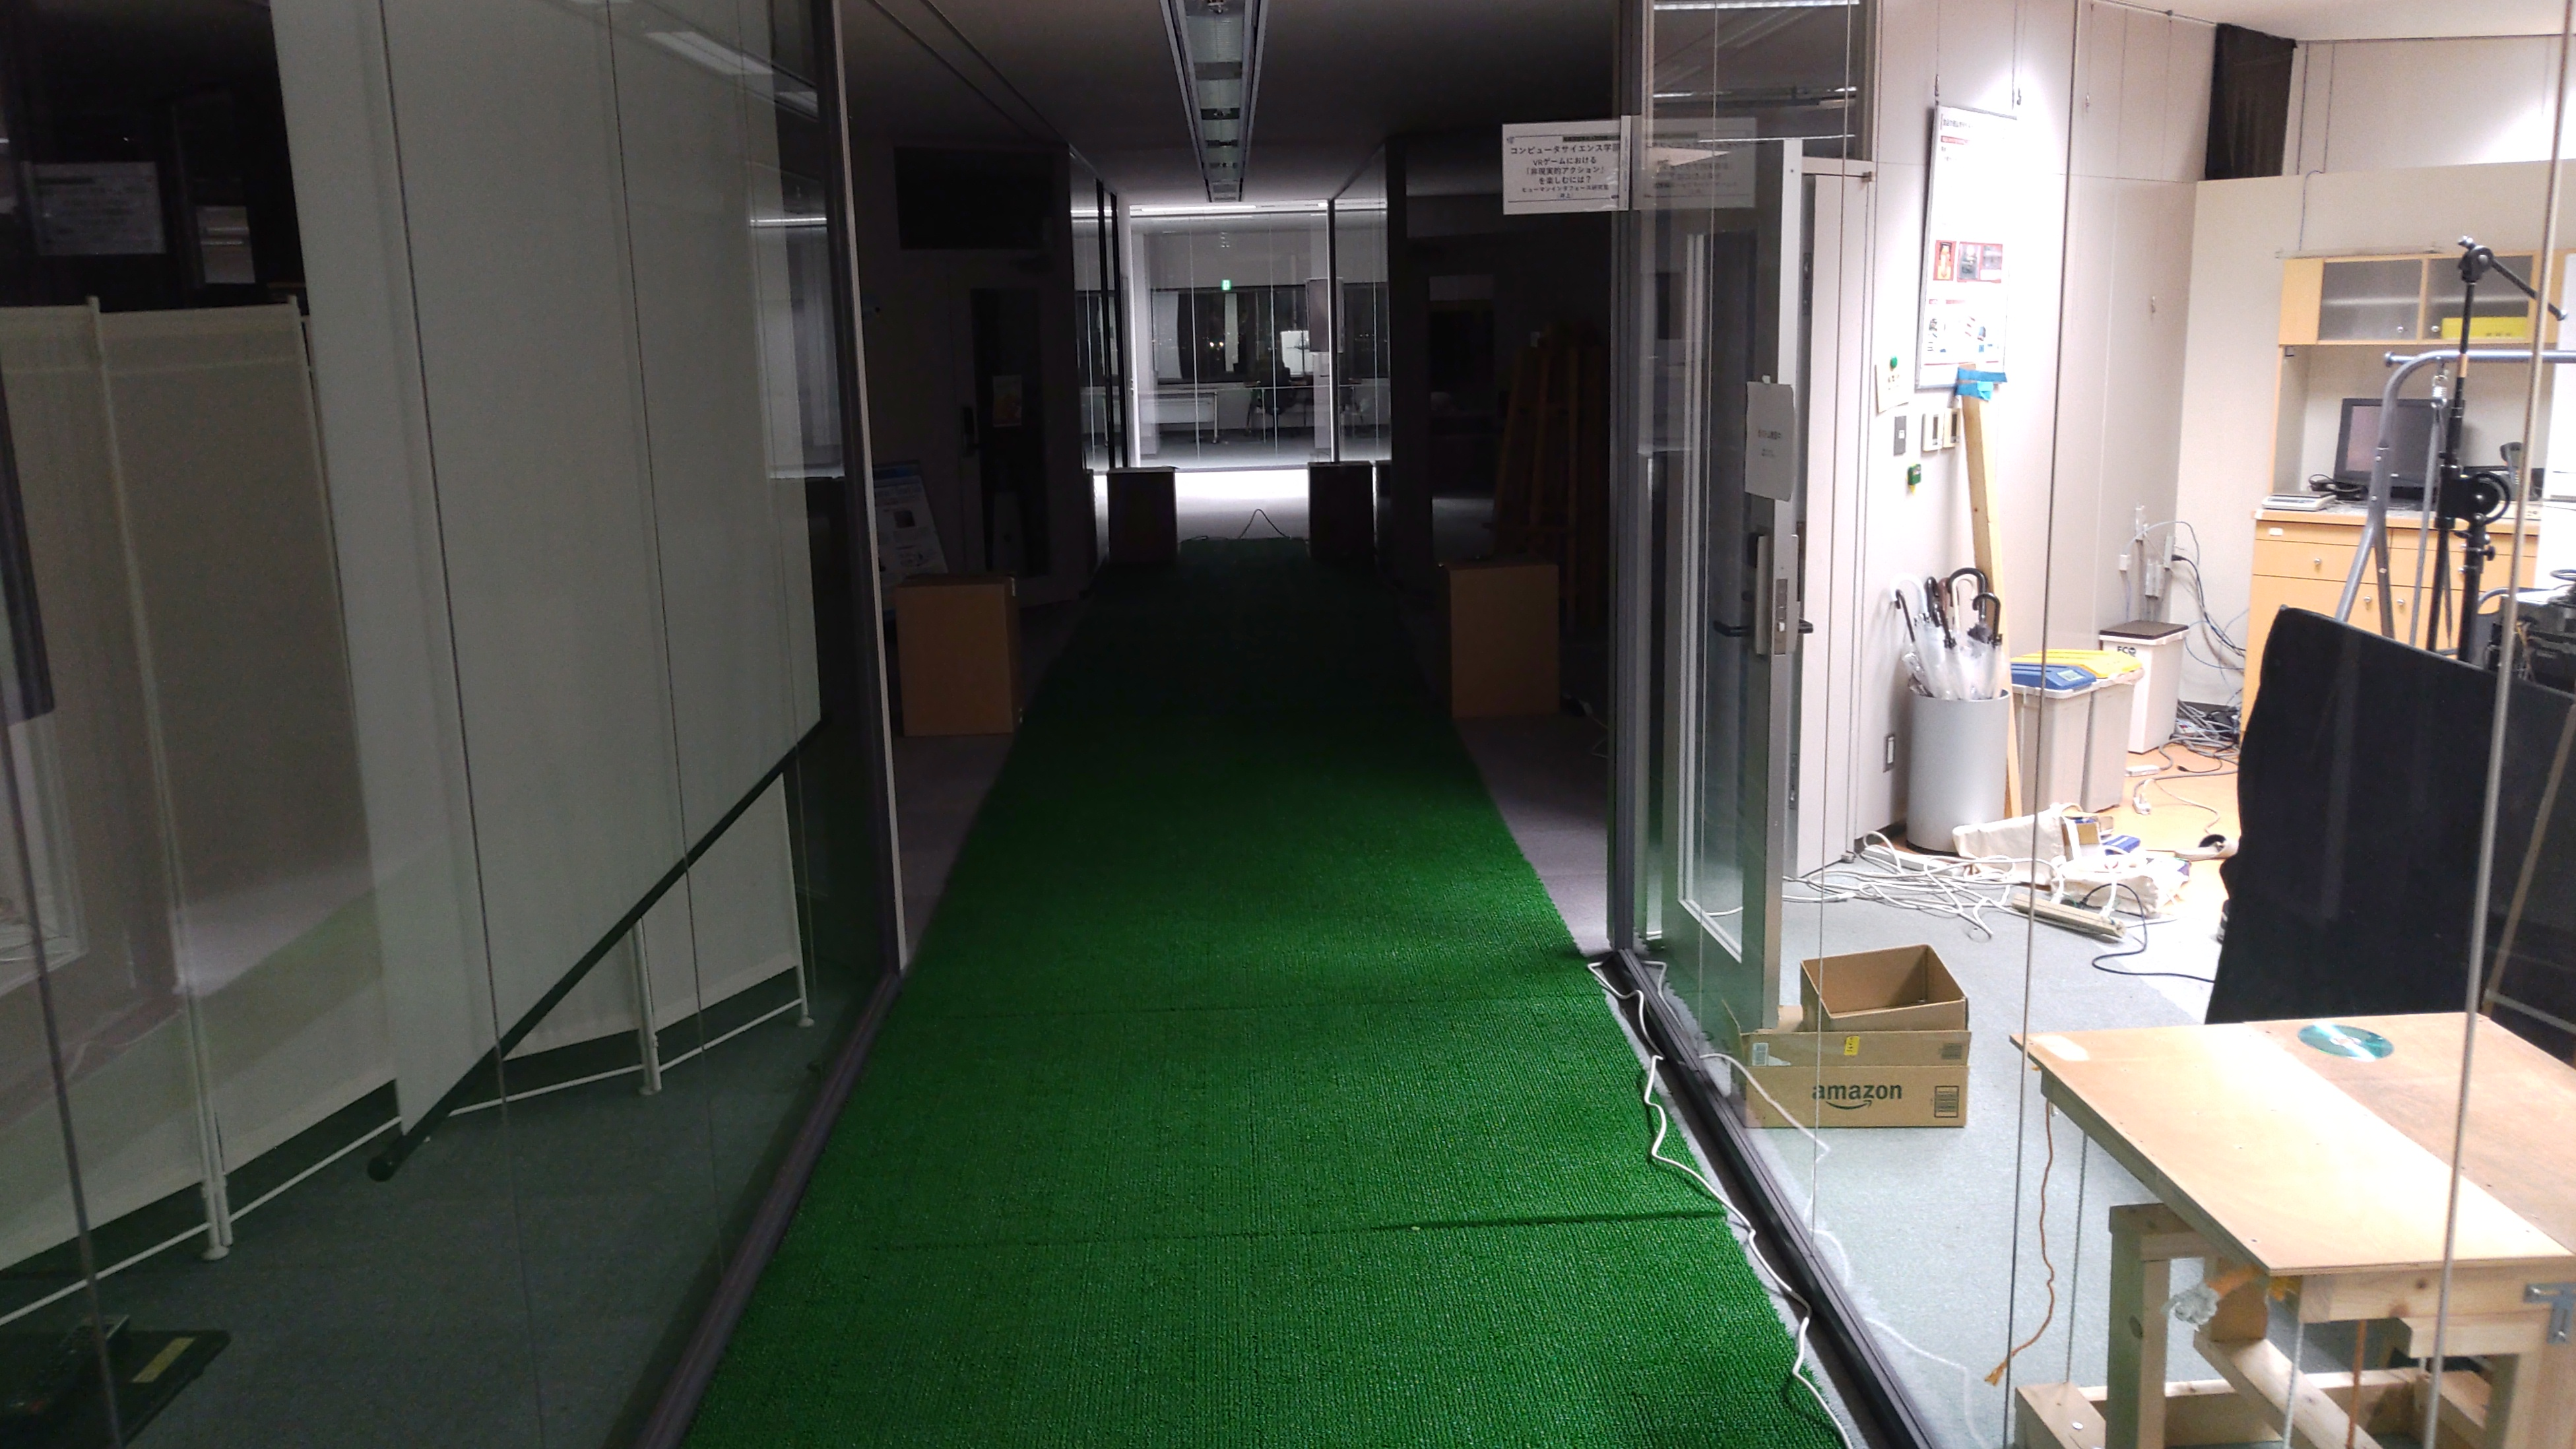
\includegraphics[width=0.7\linewidth]{fig/siten2.jpg}
    }
    \caption{実際に照明を消した実験環境}
    \label{fig:siten2}
\end{figure}

\begin{figure}[H]
    \centering
    \fbox{
        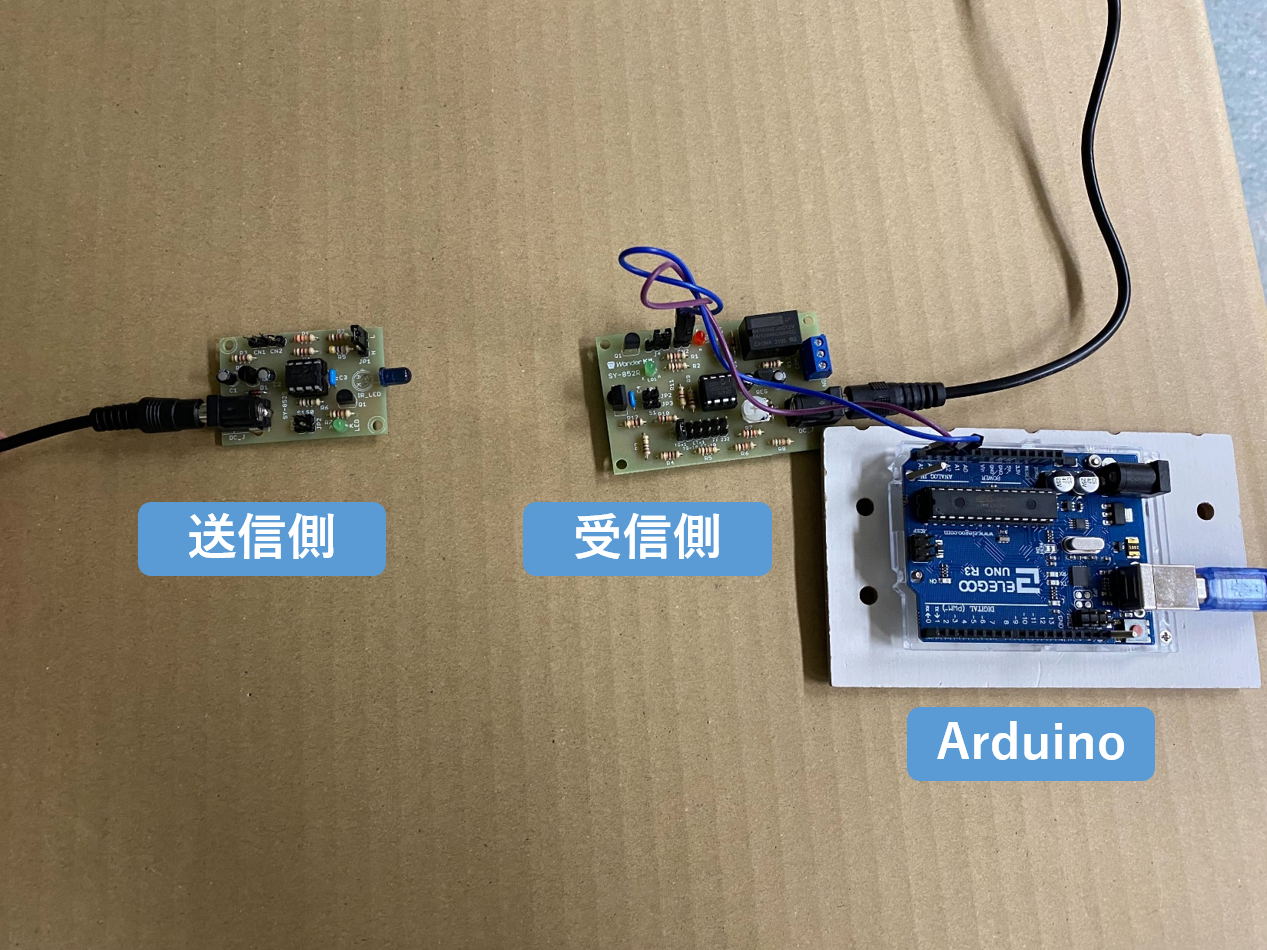
\includegraphics[width=0.7\linewidth]{fig/sensor.png}
    }
    \caption{通過センサーとArduino}
    \label{fig:13.1}
\end{figure}

\begin{figure}[H]
    \centering
    \fbox{
        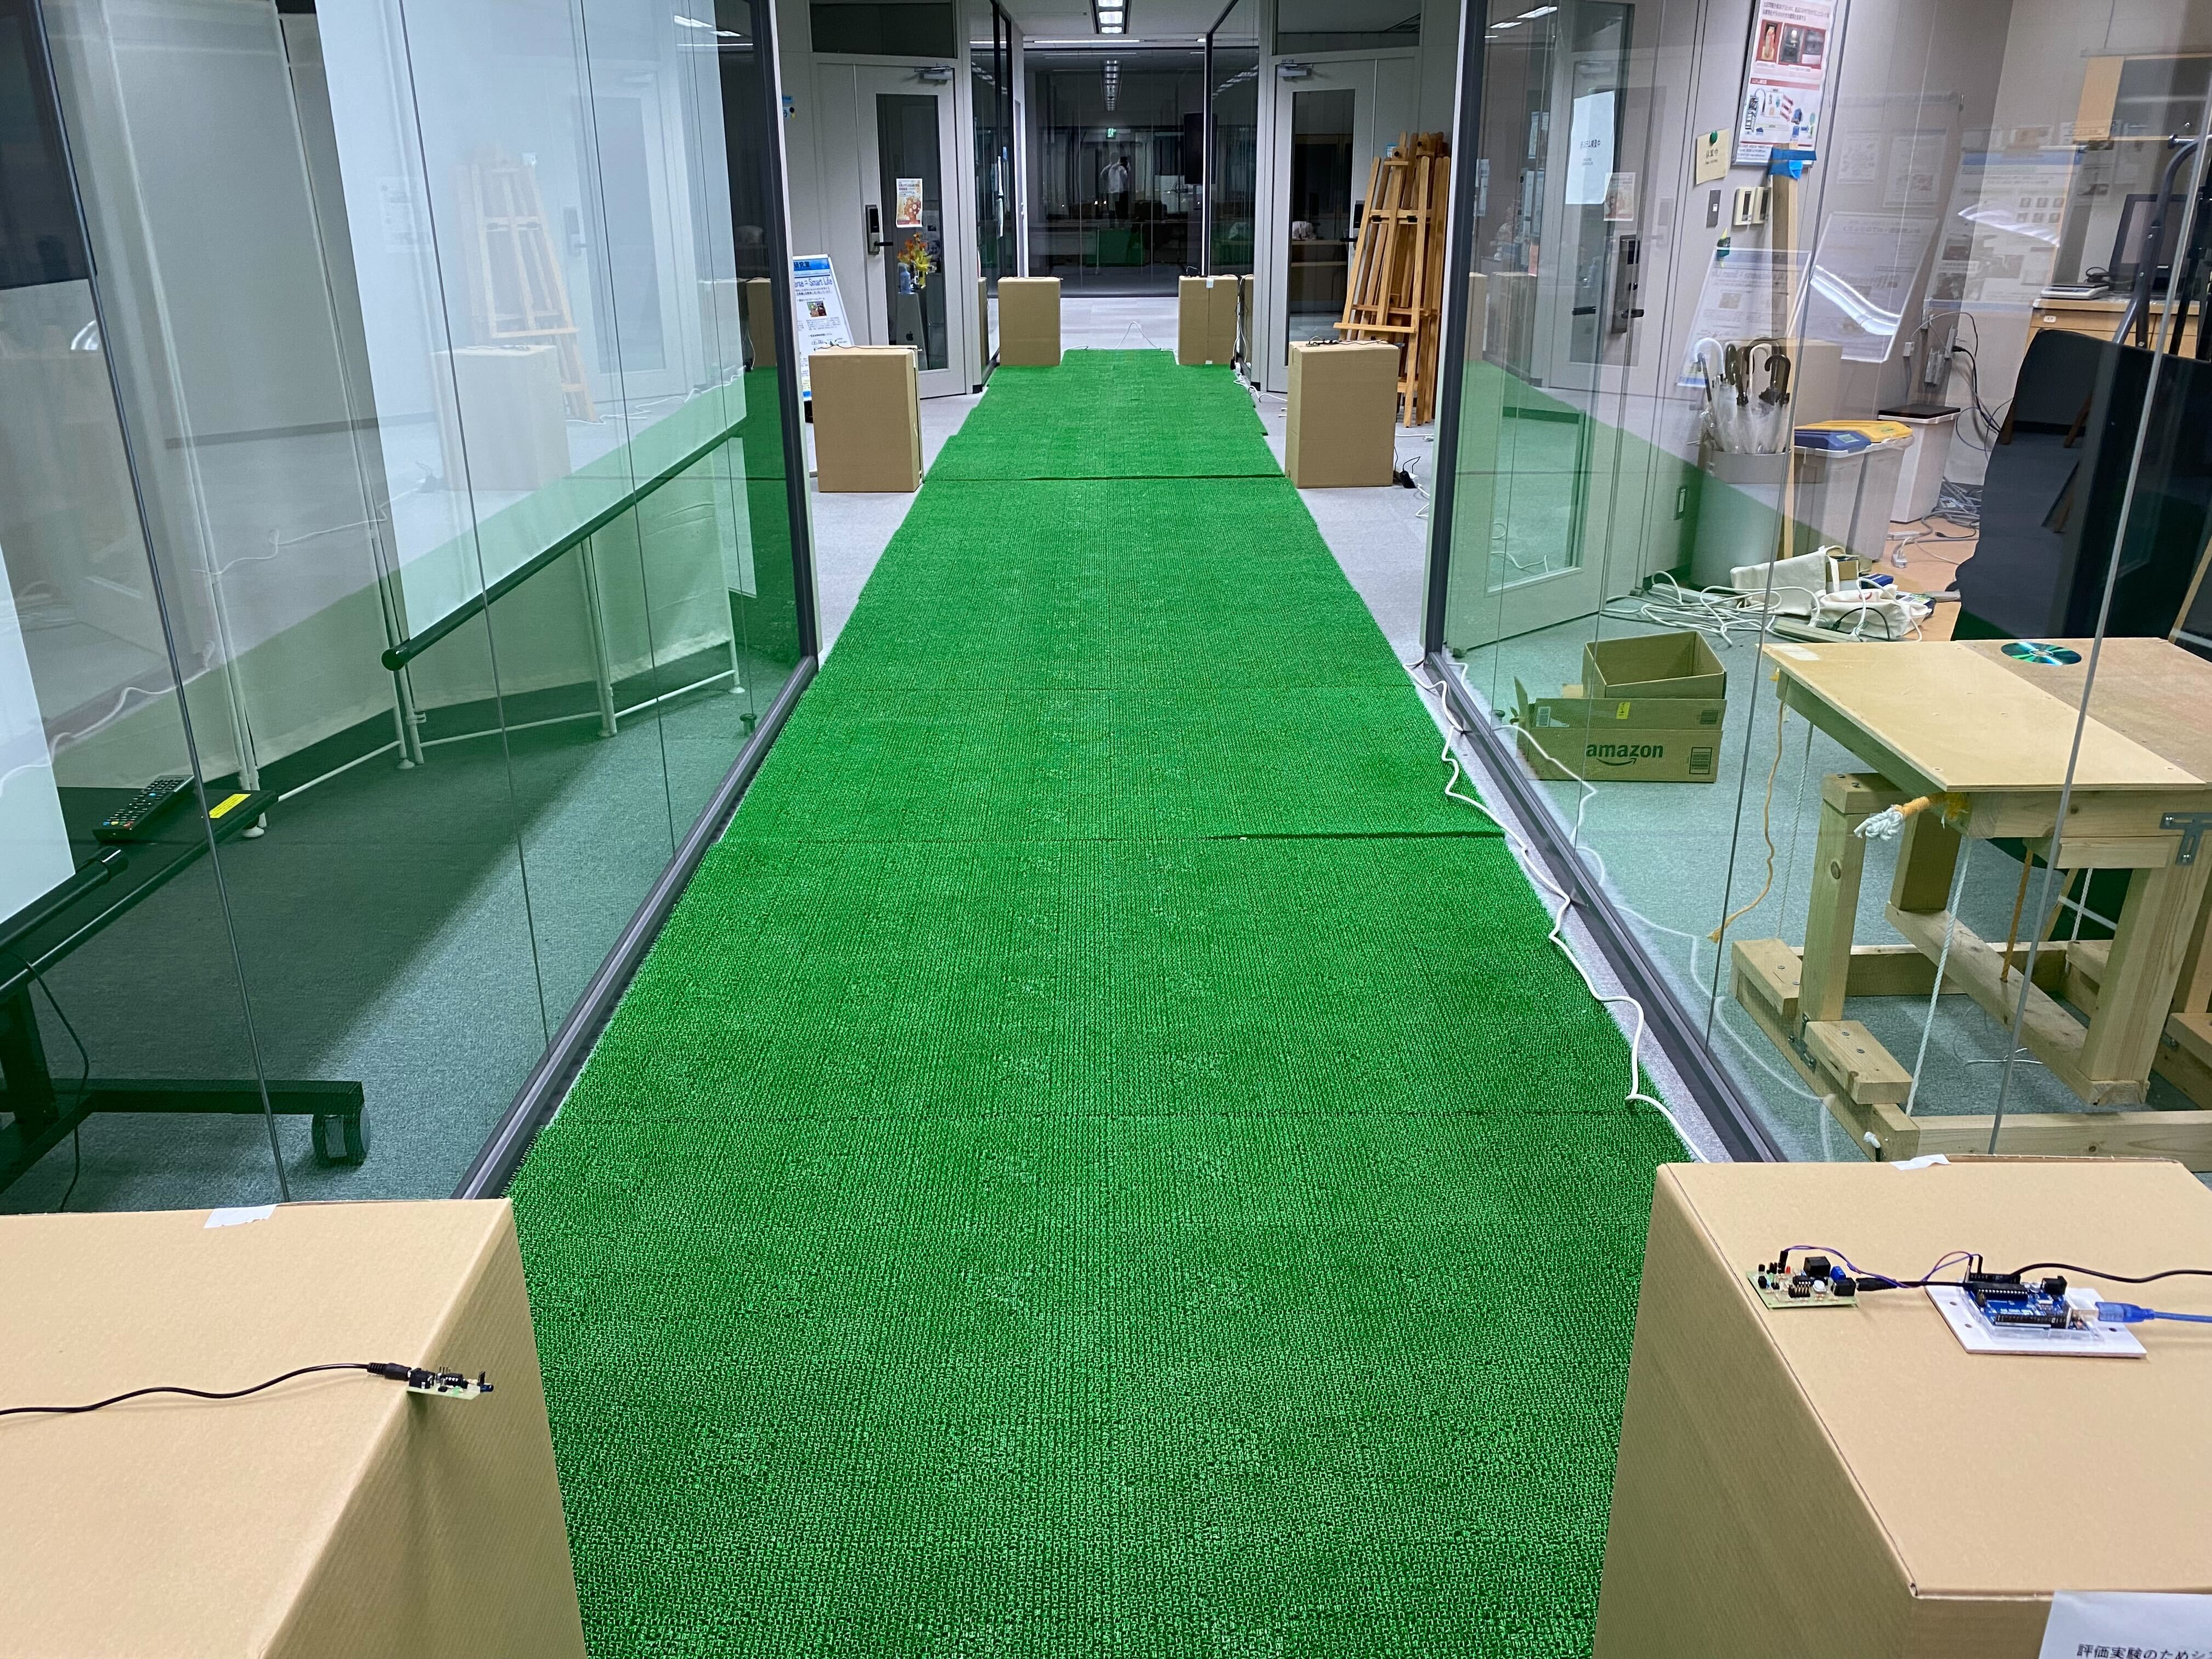
\includegraphics[width=0.7\linewidth]{fig/13.jpg}
    }
    \caption{通過センサーの配置}
    \label{fig:13}
\end{figure}



\section{実験手順}
実験手順を以下に示す.
\begin{enumerate}
    \item スタート地点に直立してもらった
    \item 指定距離歩いてもらった
    \item 歩き終わった位置で直立してもらった
\end{enumerate}
上記の手順を3回同じシステムで繰り返してもらい,それを1セットとした.
また,被験者は1セット終わるたびにアンケートを回答してもらうと共に休憩した.
この手順をシステムを使用していない状態のHoloLens2を装着した状態,
12種類のテクスチャと2種類のバーチャル床の動き方の計25セット行ってもらった.

\section{評価方法}
第4章での評価と同じく定性評価と定量評価を行う.


定性評価では,第4章でのアンケート項目に
前実験で「速く移動しているようにも感じるし,たくさん移動しているようにも感じた」というコメントがあったことから,
距離感に対しての影響の調査として
「システム未使用時に比べて歩行距離が短く感じたか」「システム未使用時に比べて歩行距離が長く感じたか」
をそれぞれ1(まったく感じなかった)~5(非常に感じた)までの5段階のリッカート尺度を用いた形で追加した.


定量評価では通過センサーを用いたタイマーから取得した時間で第4章と同じ評価方法をとる.
また,スタート地点とゴール地点の中間地点にもセンサーを置くことで中間地点での歩行時間を用いた評価も行う.
\section{実験結果}
定性評価の結果を以下に示す.
\figref{fig:f1}にシステム未使用時に比べ,バーチャル床が前から迫ってくることで速い速度感を得たか,
\figref{fig:f2}にシステム未使用時に比べ,バーチャル床が前から迫ってくることで遅い速度感を得たか
\figref{fig:f3}にシステム未使用時に比べ,バーチャル床が前から迫ってくることで歩行距離が短く感じたか,
\figref{fig:f4}にシステム未使用時に比べ,バーチャル床が前から迫ってくることで歩行距離が長く感じたか,
\figref{fig:b1}にシステム未使用時に比べ,バーチャル床が後ろから追い越してくることで速い速度感を得たか,
\figref{fig:b2}にシステム未使用時に比べ,バーチャル床が後ろから追い越してくることで遅い速度感を得たか,
\figref{fig:b3}にシステム未使用時に比べ,バーチャル床が後ろから追い越してくることで歩行距離が長く感じたか,
\figref{fig:b4}にシステム未使用時に比べ,バーチャル床が後ろから追い越してくることで歩行距離が短く感じたか,
\figref{fig:simi}にバーチャル床は本物の床が動いているように見えたかのアンケート結果を示す.
これらの棒グラフは,左から1(まったく感じなかった)~5(非常に感じた),円グラフでは1(まったく見えなかった)~5(非常に見えた)となっている.
バーチャル床が前から迫ってくる場合,
\figref{fig:f1},\figref{fig:f2}から,5YR天然のテクスチャ(\figref{fig:ff5yr})が一番速い速度感を与えることがわかり,バーチャル床が前から迫ってく表示の仕方をするとどのテクスチャも遅い速度感を与えないということが分かった.
\figref{fig:f3},\figref{fig:f4}から,体感歩行距離が短く感じることはどのテクスチャでもなかったが,5G天然(\figref{fig:fl5G})と5B砂利(\figref{fig:fl5B})は歩行距離を長く感じさせる効果があるとわかった.
バーチャル床が後ろから追い越してくる場合では,
\figref{fig:b1},\figref{fig:b2}から,バーチャル床が後ろから追い越してくることで,速い速度感は与えないことがわかった.しかし,5YR人工(\figref{fig:bs5YR})は遅い速度感を与えることがわかった.
また,\figref{fig:b3},\figref{fig:b4}から,ほとんどのテクスチャは体感歩行距離に影響を与えないことがわかった.
\figref{fig:simi}から,5RP天然(\figref{fig:c5RP})がもっとも本物の床が動いているように見えてということがわかった.
\begin{figure}[H]
    \centering
    \fbox{
        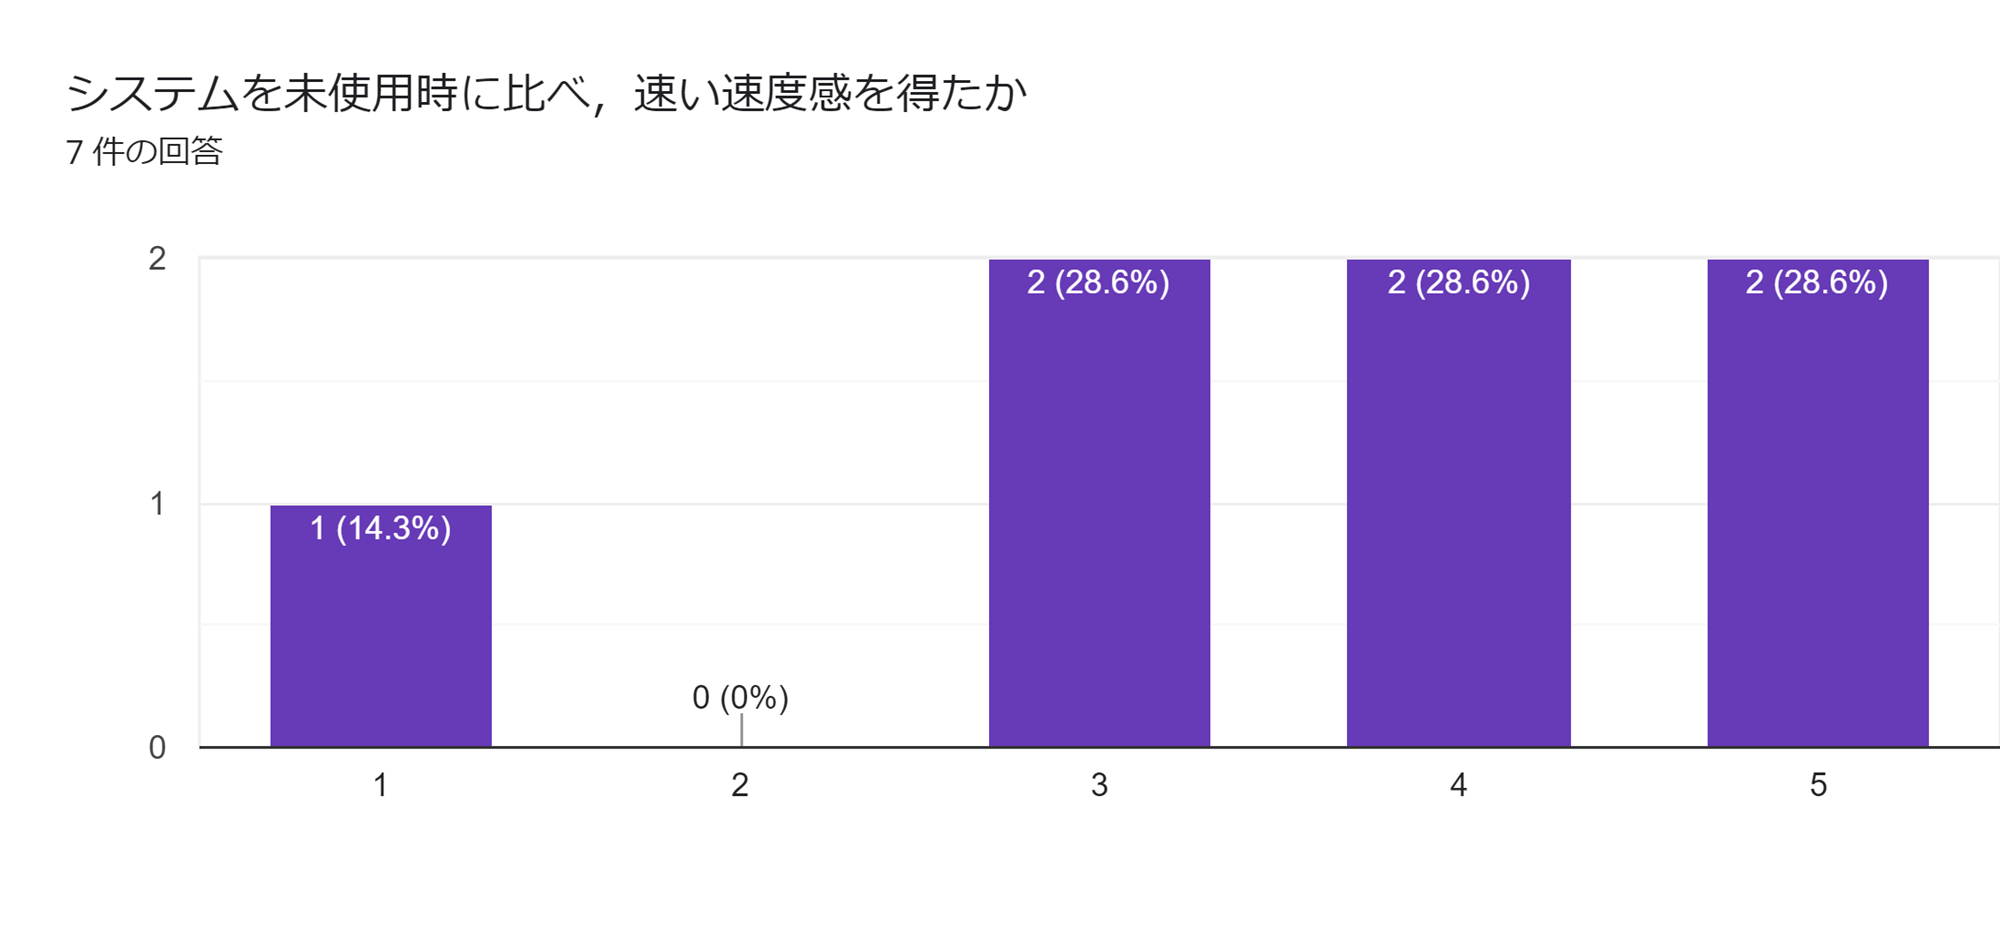
\includegraphics[width=0.8\linewidth]{fig/前早5YR天然.png}
    }
    \caption{システム未使用時に比べ,バーチャル床が前から迫ってくることで速い速度感を得たかの結果(5YR天然)}
    \label{fig:ff5yr}
\end{figure}
\begin{figure}[H]
    \centering
    \fbox{
        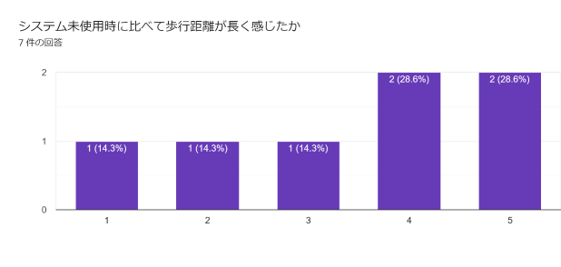
\includegraphics[width=0.8\linewidth]{fig/前長5G天然.png}
    }
    \caption{システム未使用時に比べ,バーチャル床が前から迫ってくることで歩行距離が長く感じたかの結果(5G天然)}
    \label{fig:fl5G}
\end{figure}

\begin{figure}[H]
    \centering
    \fbox{
        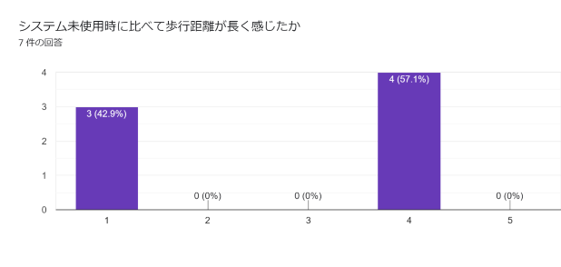
\includegraphics[width=0.8\linewidth]{fig/前長5B砂利.png}
    }
    \caption{システム未使用時に比べ,バーチャル床が前から迫ってくることで歩行距離が長く感じたかの結果(5B砂利)}
    \label{fig:fl5B}
\end{figure}

\begin{figure}[H]
    \centering
    \fbox{
        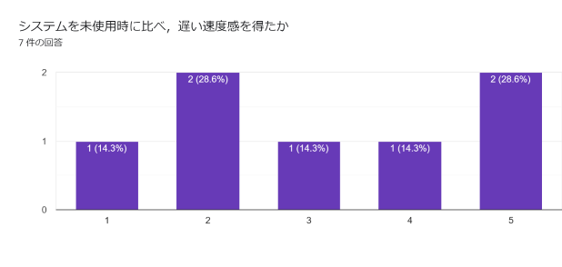
\includegraphics[width=0.8\linewidth]{fig/後遅5YR人工.png}
    }
    \caption{システム未使用時に比べ,バーチャル床が後ろから追い越してくることで遅い速度感を得たかの結果(5YR人工)}
    \label{fig:bs5YR}
\end{figure}

\begin{figure}[H]
    \centering
    \fbox{
        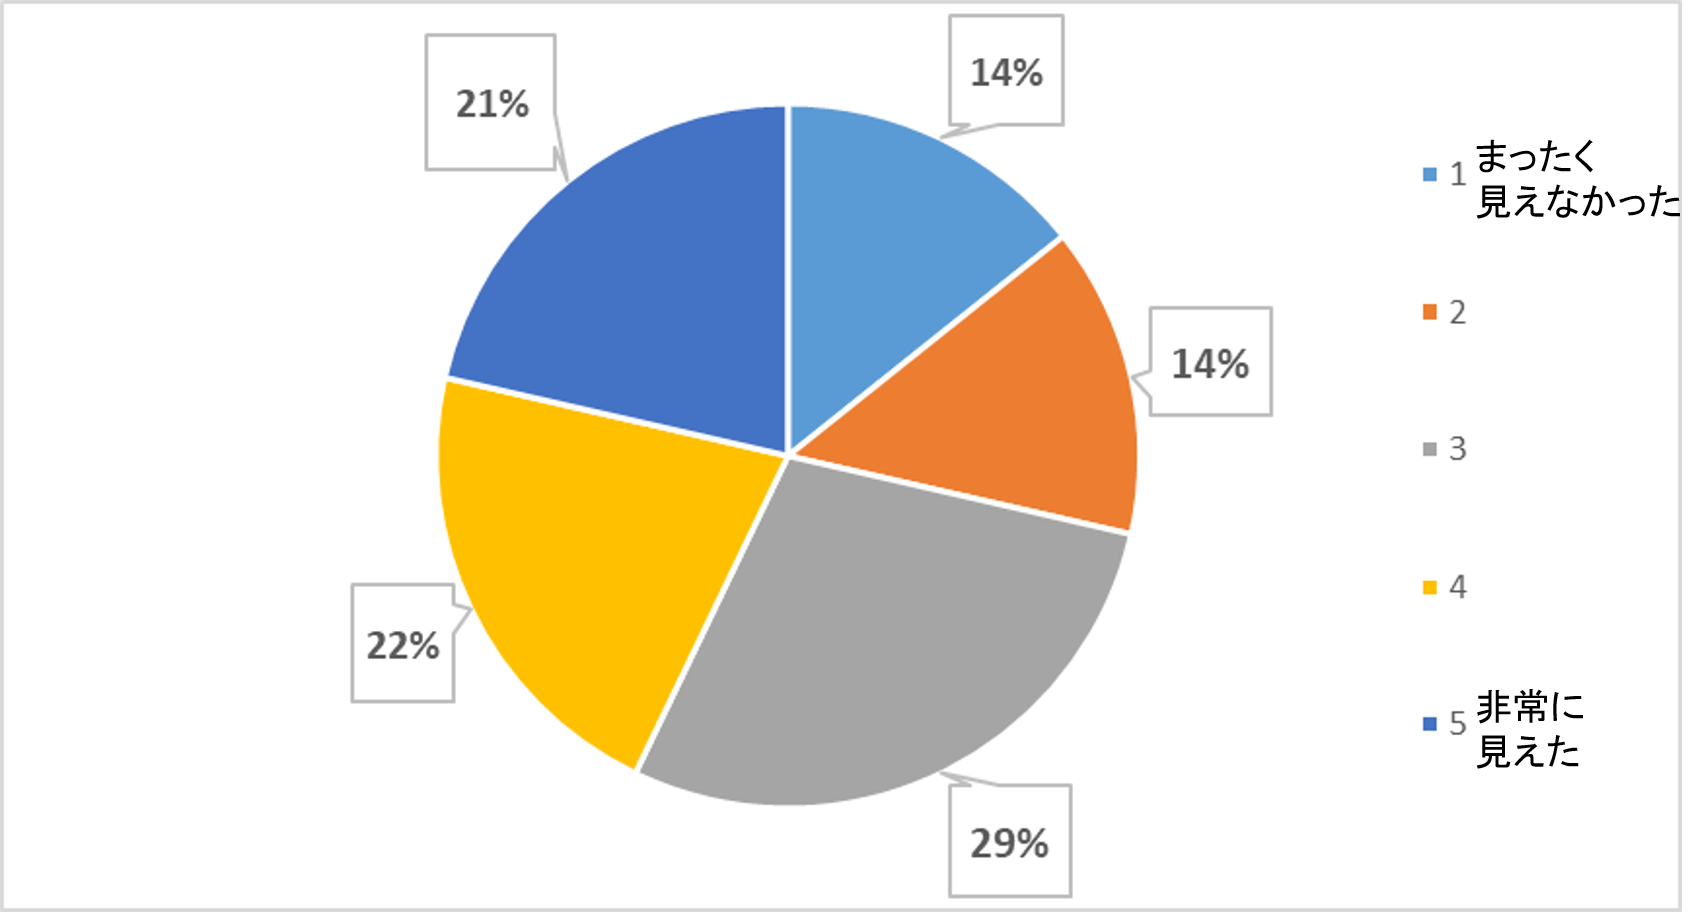
\includegraphics[width=0.8\linewidth]{fig/色5RP天然.png}
    }
    \caption{バーチャル床は本物の床が動いているように見えたかの結果(5RP天然)}
    \label{fig:c5RP}
\end{figure}

定量評価の結果を以下に示す.
\figref{fig:maehalf}にシステム未使用時とバーチャル床が前から迫ってくるシステム使用時の中間地点までの時間差の一覧,
\figref{fig:maetime}にシステム未使用時とバーチャル床が前から迫ってくるシステム使用時のゴールまでの時間差の一覧.
\figref{fig:usirohalf}にシステム未使用時とバーチャル床が後ろから追い越してくるシステム使用時の中間地点までの時間差一覧.
\figref{fig:usirotime}にシステム未使用時とバーチャル床が後ろから追い越してくるシステム使用時のゴールまでの時間差一覧を示す.
バーチャル床が前から迫ってくる場合,
\figref{fig:maehalf}から,中間地点では被験者によって時間の差はプラスマイナスが分かれたが
\figref{fig:maetime}から,5YR人工(\figref{fig:5YRjinko})とリアルテクスチャである5G人工(\figref{fig:5Gjinko})はゴールまでの歩行時間が長くなっていた.

バーチャル床が後ろから追い越してくる場合では,
\figref{fig:usirohalf}から,中間地点では被験者によって時間の差はプラスマイナスが分かれた.
しかし,\figref{fig:usirotime}から,5YR天然(\figref{fig:5YRten}),5RP天然(\figref{fig:5RPten}),5RP人工(\figref{fig:5RPjinko}),ではゴール時の全ユーザが歩行時間が短くなっていた.
これらの結果は,SSQによる映像酔いの調査結果からの影響は確認できなかった.
\begin{figure}[H]
    \centering
    \fbox{
        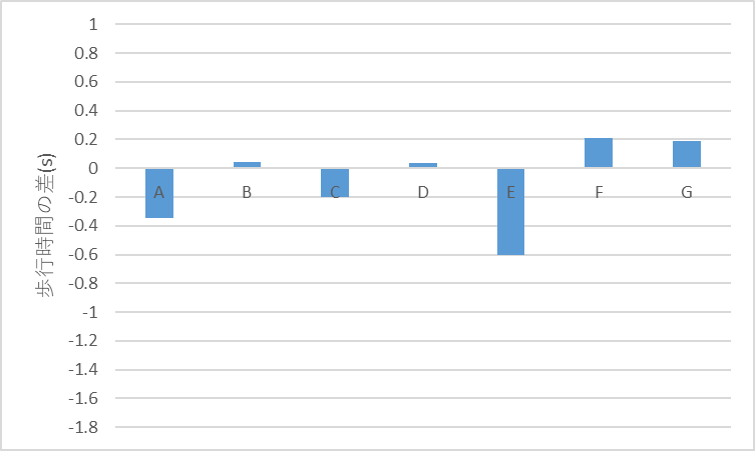
\includegraphics[width=0.8\linewidth]{fig/前速度早5YR人工.png}
    }
    \caption{システム未使用時とバーチャル床が前から迫ってくるシステム使用時のゴールまでの時間差(5YR人工)}
    \label{fig:5YRjinko}
\end{figure}

\begin{figure}[H]
    \centering
    \fbox{
        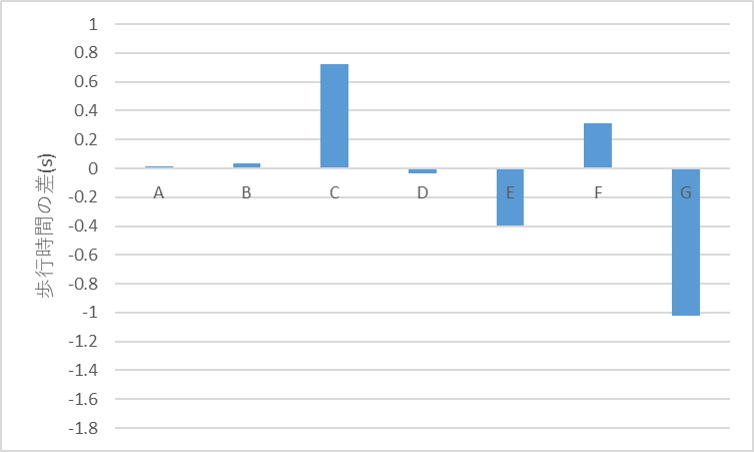
\includegraphics[width=0.8\linewidth]{fig/前速度早5G人工.png}
    }
    \caption{システム未使用時とバーチャル床が前から迫ってくるシステム使用時のゴールまでの時間差(5G人工)}
    \label{fig:5Gjinko}
\end{figure}

\begin{figure}[H]
    \centering
    \fbox{
        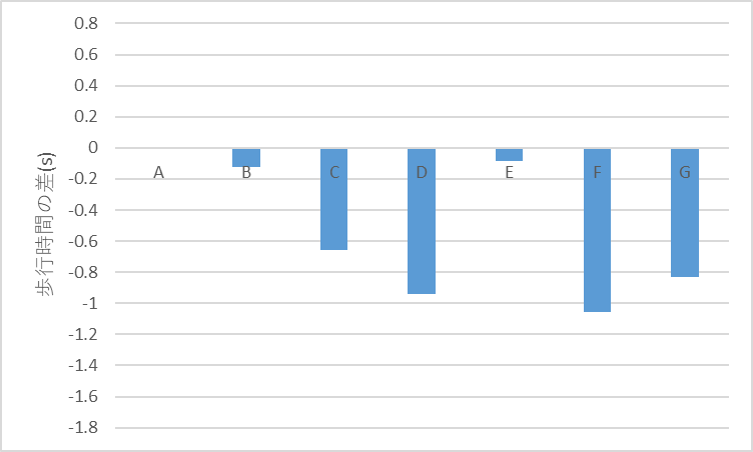
\includegraphics[width=0.8\linewidth]{fig/後速度早5YR天然.png}
    }
    \caption{システム未使用時とバーチャル床が後ろから追い越してくるシステム使用時のゴールまでの時間差(5YR天然)}
    \label{fig:5YRten}
\end{figure}

\begin{figure}[H]
    \centering
    \fbox{
        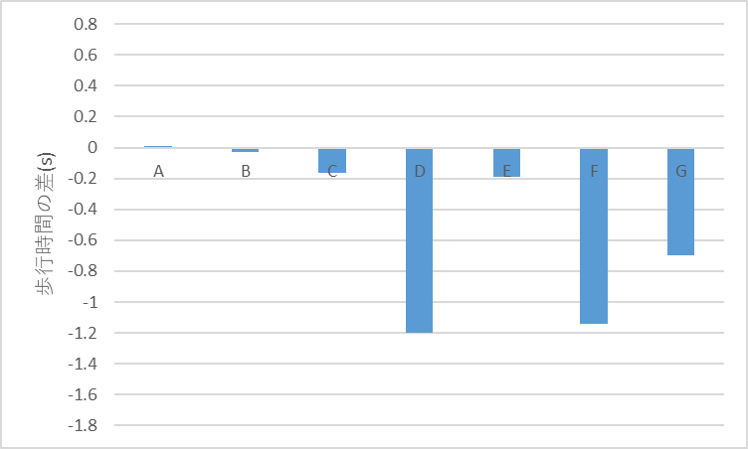
\includegraphics[width=0.8\linewidth]{fig/後速度早5RP天然.png}
    }
    \caption{システム未使用時とバーチャル床が後ろから追い越してくるシステム使用時のゴールまでの時間差(5RP天然)}
    \label{fig:5RPten}
\end{figure}

\begin{figure}[H]
    \centering
    \fbox{
        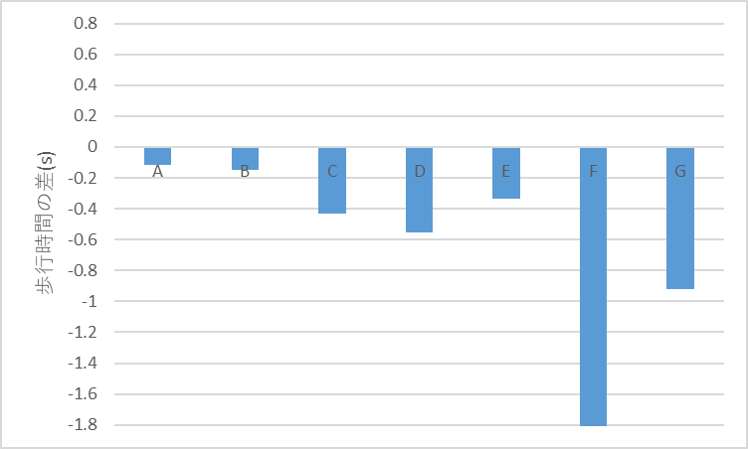
\includegraphics[width=0.8\linewidth]{fig/後速度早5RP人工.png}
    }
    \caption{システム未使用時とバーチャル床が後ろから追い越してくるシステム使用時のゴールまでの時間差(5RP人工)}
    \label{fig:5RPjinko}
\end{figure}


\section{考察}
今回仮説としてユーザの行動制御ができると考えていたリアルテクスチャは,効果が無かったことから,
ユーザに対してバーチャル床が見えやすい状態では実際の床にテクスチャを近似させる効果はないことが考察できた.
しかし,「砂利が一番好き.現実空間の床を消せてる.」や「砂利が模様が一番わかりやすかった」というコメントから実際の床にテクスチャを近似させるよりも
動いていることが分かりやすいテクスチャを作るほうが重要だと考察できる.


バーチャル床が後ろからユーザを追い越す動きをした場合,5YR人工は遅い速度感を与えることはできたが他のテクスチャは何も与えられなかった.
しかし,5YR天然,5RP人工,そして一番最も本物の床に見られていた5RP天然は定量評価の結果,システム未使用時に比べ,歩行時間が短くなっていた.
これらは共通して実際の床の色と色相環で見て,反対に位置する色が多い.
このことから色は現実の床と近似させないことで効果が強まると考えられる.
また,このバーチャル床の動かし方は上記の結果から
速度感を低下させ,ユーザの歩行速度を上昇させる効果があると考察できる.


バーチャル床が前から迫ってくる場合,遅い速度感を与えることはできなかったが,5YR天然は速い速度感を与えることには成功した.
さらに,定量評価の結果から,5YR人工とリアルテクスチャである5G人工は半数以上の被験者が歩行速度が低下していた.
これにより,床と同じ模様バーチャル床を前から迫ってくる動かし方は速度感を上昇させ,ユーザの歩行速度を遅くさせることが示唆された.
5G天然と5B砂利は体感歩行距離を長くしていたことから,テクスチャによってはこのバーチャル床の動き方は距離感に影響を与えることが示唆された.


これらの結果から,中間地点では歩行時間のプラスマイナスは分かれていたにもかかわらず,ゴール地点では
歩行時間が短くなっていたことから,本システムは一定時間経過後に効果が出始めることが考えられる.
しかし,今回の実験では効果が衰退し始めるタイミングはわからなかった.
今回のシステムはシースルー型のHMDを使用したため,ビデオスルー型のHMDを使用した場合ではバーチャル床の見え方が変わることが想定できるため
効果が変わってくることも考えられた.
	% 第5章 評価
\chapter{結論}
本研究では,
ユーザの視界に映る床に現実の床を模したバーチャル床をアニメーション重畳表示するシステムである
TravelatARを提案し,ユーザの歩行速度を制御することを目的に評価実験を行った.


実験の結果,本システムは一定時間経過後に効果が出始めること,
「5YR天然」,「5RP天然」,「5RP人工」のテクスチャを用いたバーチャル床を
後ろからユーザを追い越す動きでアニメーション重畳表示することで「ユーザの歩行速度を早くする」と「システム未使用時に比べ遅い速度感を与えること」が示唆された.


本研究ではシースルー型のHMDを用いて実験していたが,
ビデオスルー型のHMDを用いた場合ではバーチャル床の見え方が変わり,効果が変わると仮説を立てた.
だが,新型ビデオスルー型のHMDで開発を行った際,深度カメラのAPIが公開されていなかったため,実装,実験を行えなかった\cite{ocu}.
そのため,今後の課題としてビデオスルー型のHMDでの効果を確認する必要があると考える.

今後の展望として,今回仮説としてユーザの行動制御ができると考えていたリアルテクスチャは,効果が無かったが
リアルテクスチャにも動いている目安となるものを加えることで効果が強まることが考えられる.	% 第6章 結論
% acknowlegments.tex -- 謝辞
\theacknowledgments
本研究を進めるにあたり井上亮文 准教授をはじめとした皆様からご指導,ご意見を頂きましたことに心より御礼申し上げます.
B4の頃からを含め3年間苦楽を共にした荒川,ためになる話をたくさんしてくれた最強の先輩であるリズキー先輩,
実験を手伝ってくれたり,愉快な話をしてくれた室井君,市川君,武田君,川東君,
卒業後も支えてくれた池田,田中.
最後になりましたが,日常の議論を通じて多くの知識や示唆を頂いた井上研究室の皆様に御礼申し上げます.ありがとうございました.		% 謝辞
\bibliographystyle{junsrt}
\bibliography{mybib} % 参考文献
%
% 自分の名前の下に下線を引いても良いかもしれません
%

\begin{theachievement}{99}
  \bibitem{DCC2022} 島谷優佑, 井上亮文, "歩行移動時の運動量を増加させるARステップ誘導システムの検討", 情報処理学会研究報告デジタルコンテンツクリエーション(DCC), Vol. 2022-DCC-32, No.12, pp.1-5, 2022年11月.
  \bibitem{DCC2023}島谷優佑, 井上亮文, "travelatAR:地表面近似テクスチャーのアニメーション重畳表示による歩行速度制御システム", 情報処理学会研究報告デジタルコンテンツクリエーション(DCC), Vol.2023-DCC-35, No.6, pp.1-6, 2023年11月.
\end{theachievement}
 % 業績
% appendix.tex -- 付録
\appendix
\chapter{追加実験結果}
追加実験の結果を以下に示す.
\begin{figure}[H]
    \centering
    \fbox{
        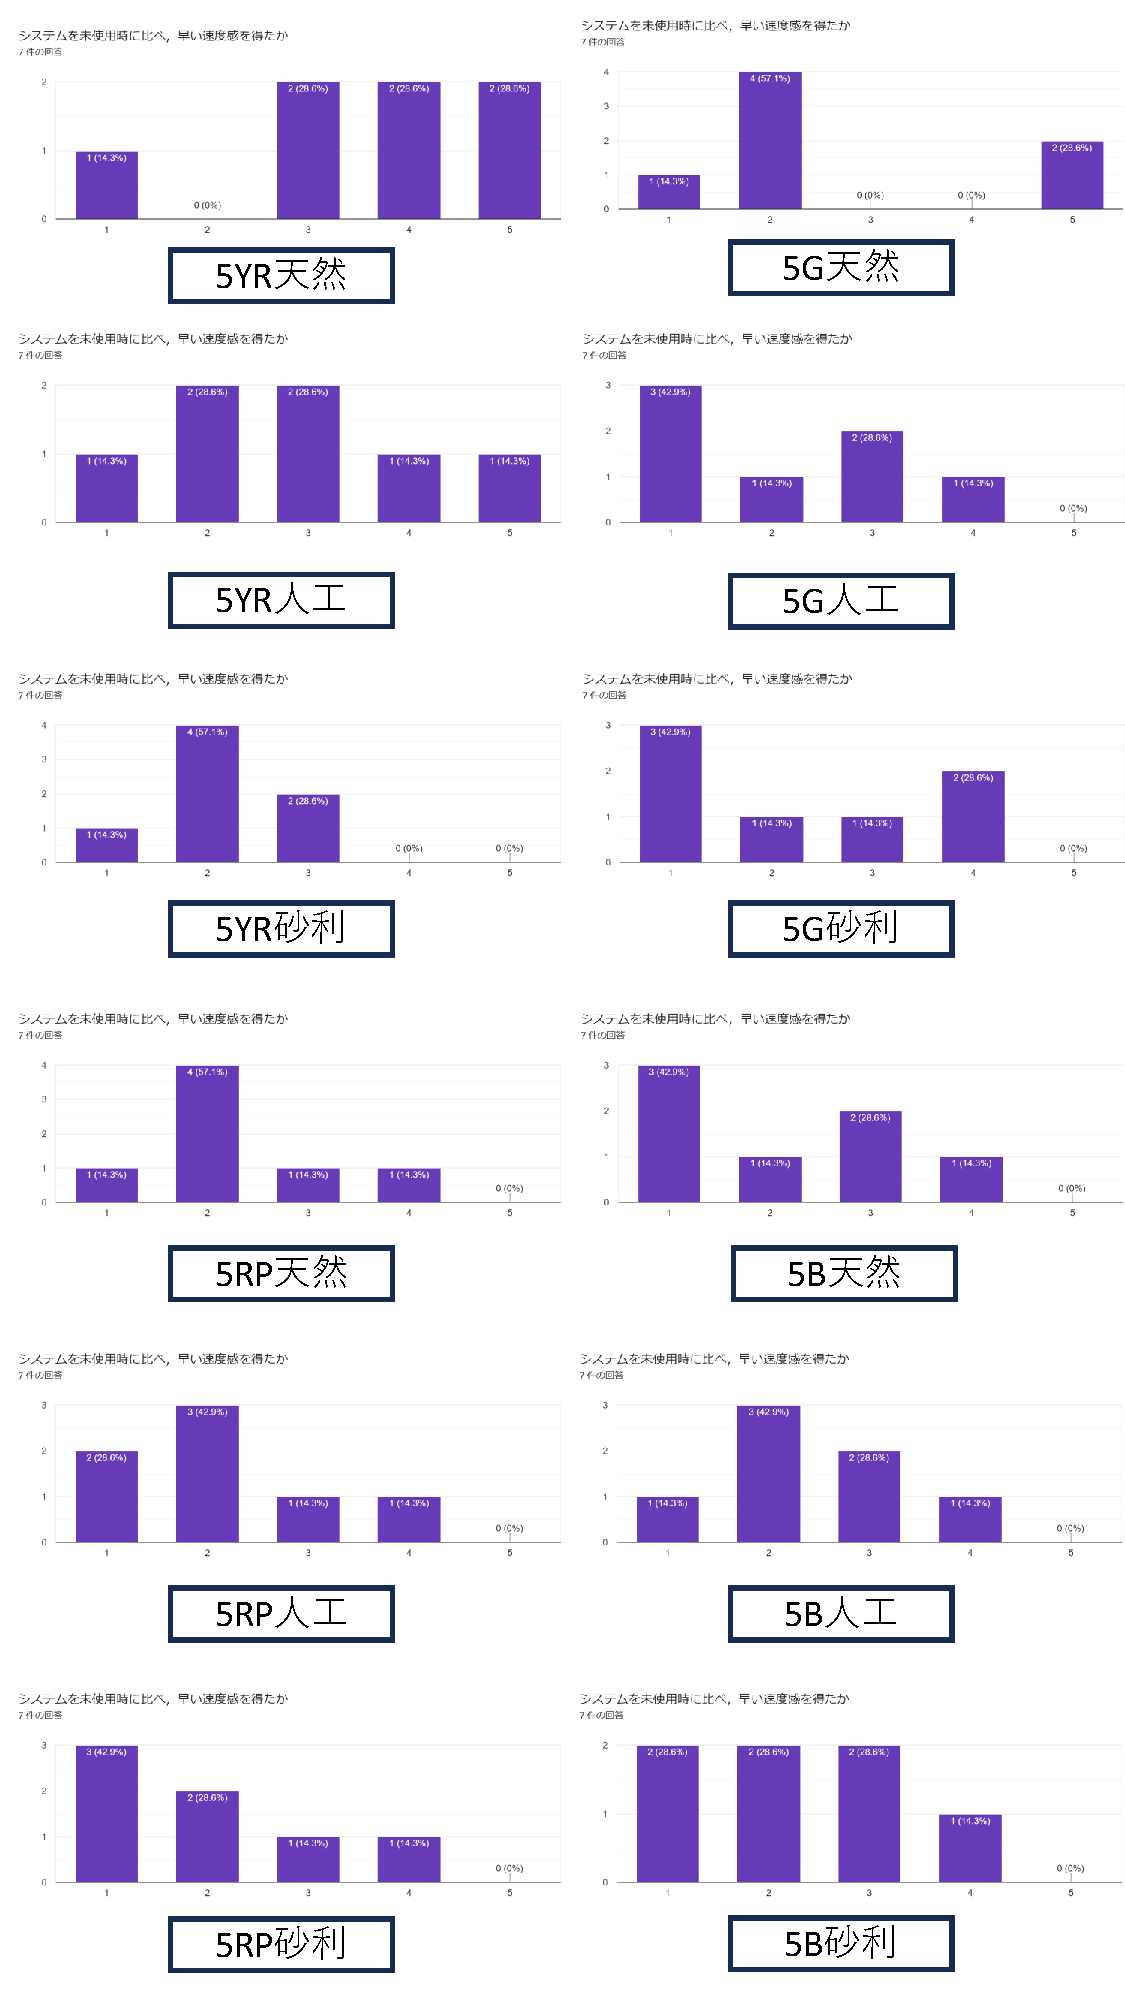
\includegraphics[width=0.8\linewidth]{fig/(前)faster.pdf}
    }
    \caption{バーチャル床が前から迫ってくることで早い速度感を得たかのアンケート結果}
    \label{fig:f1}
\end{figure}
\begin{figure}[H]
    \centering
    \fbox{
        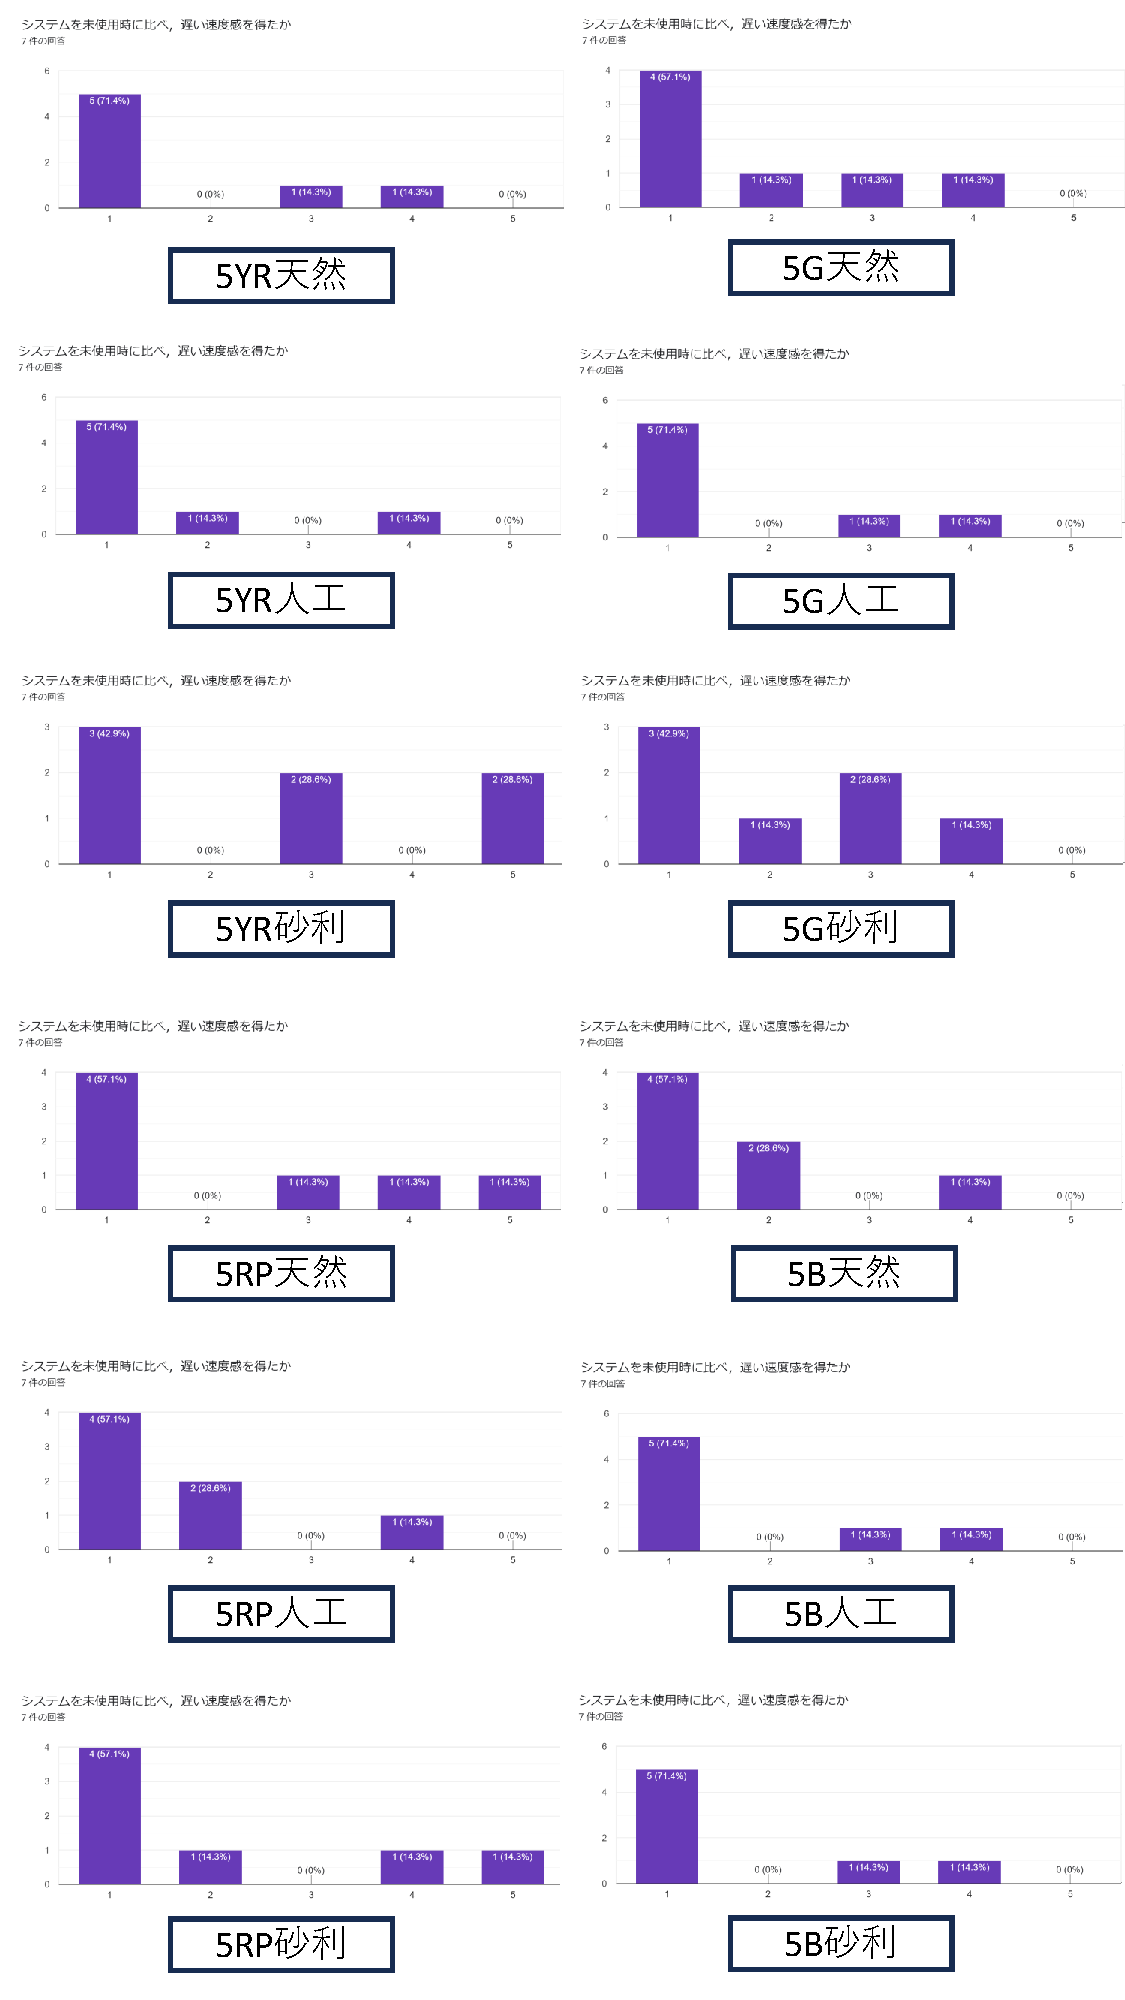
\includegraphics[width=0.8\linewidth]{fig/(前)slower.pdf}
    }
    \caption{バーチャル床が前から迫ってくることで遅い速度感を得たかのアンケート結果}
    \label{fig:f2}
\end{figure}
\begin{figure}[H]
    \centering
    \fbox{
        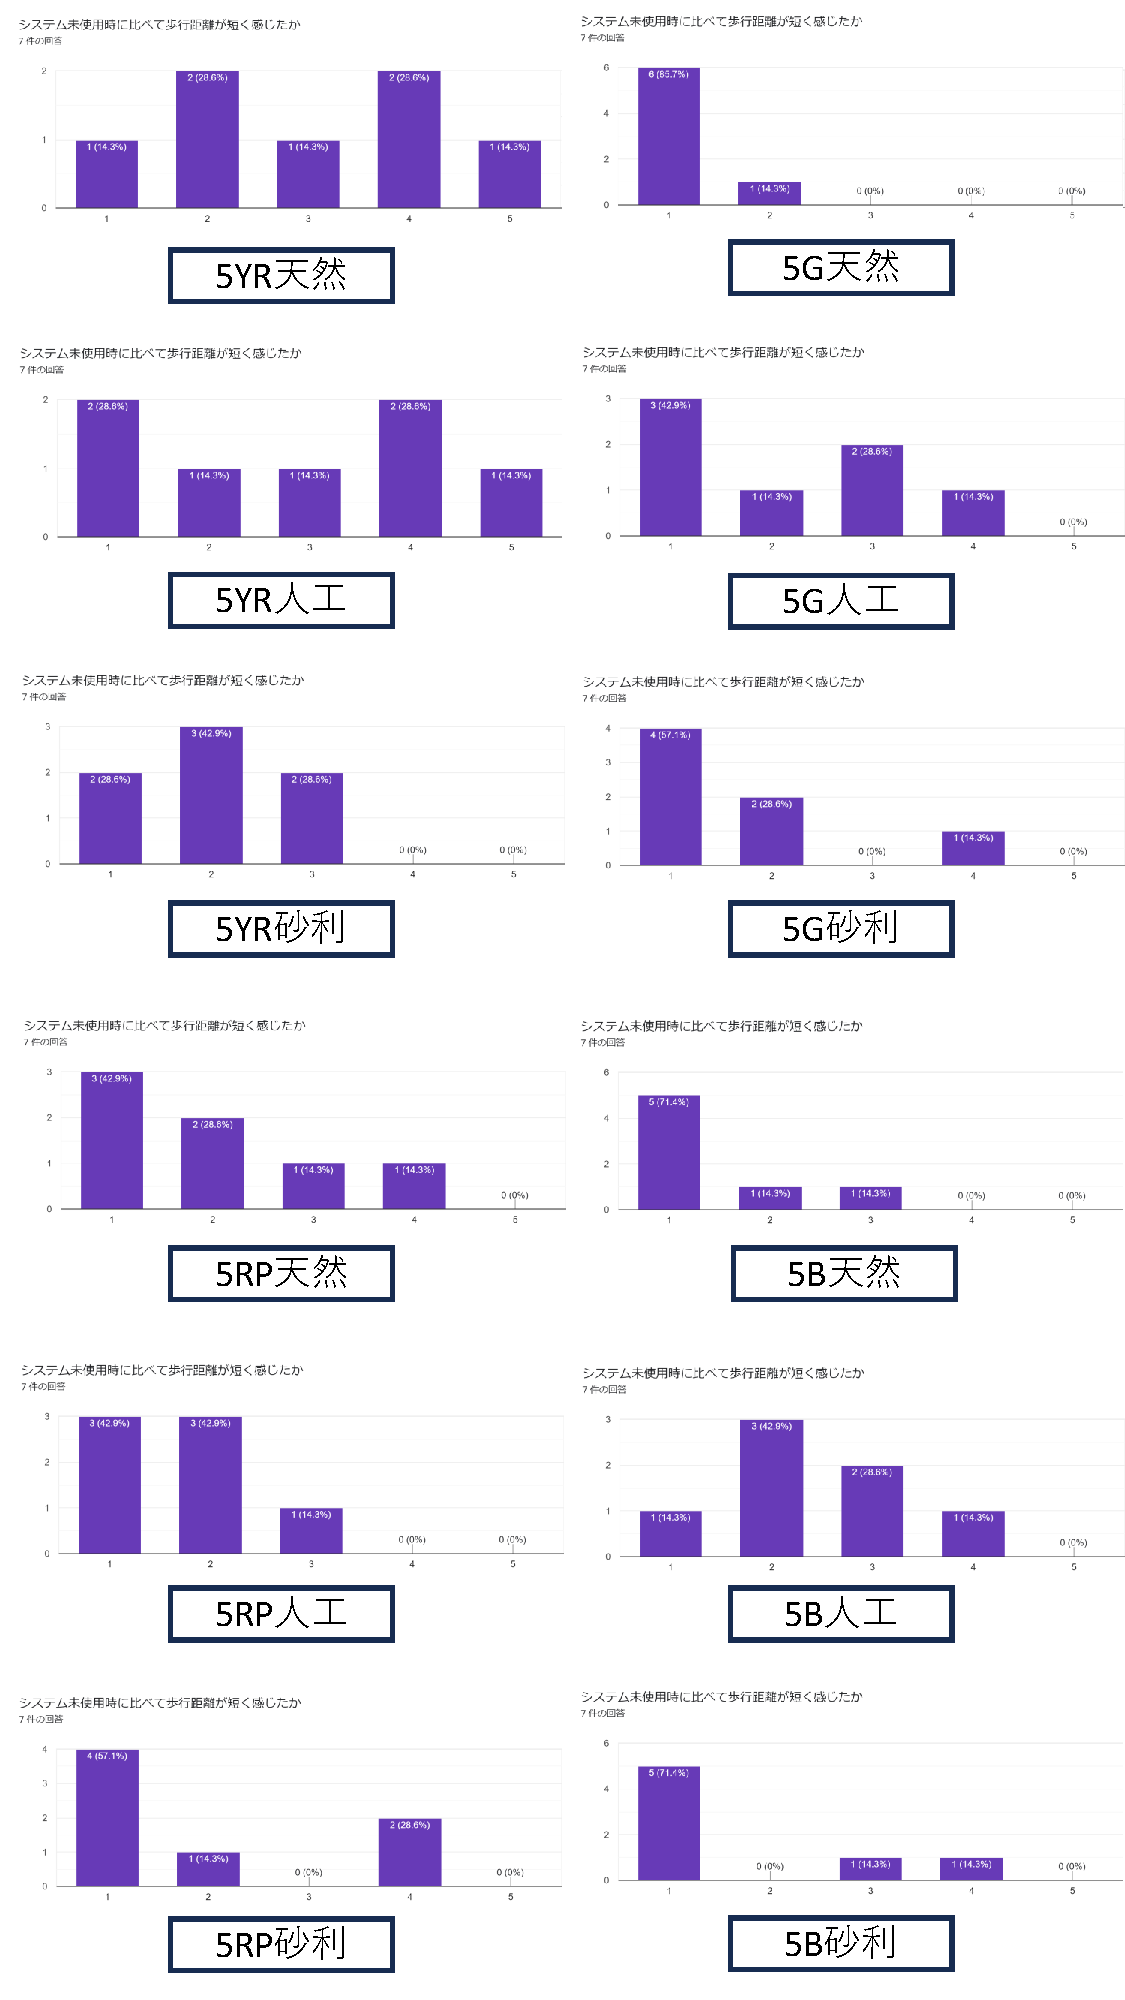
\includegraphics[width=0.8\linewidth]{fig/(前)shoater.pdf}
    }
    \caption{バーチャル床が前から迫ってくることで歩行距離が短く感じたかのアンケート結果}
    \label{fig:f3}
\end{figure}
\begin{figure}[H]
    \centering
    \fbox{
        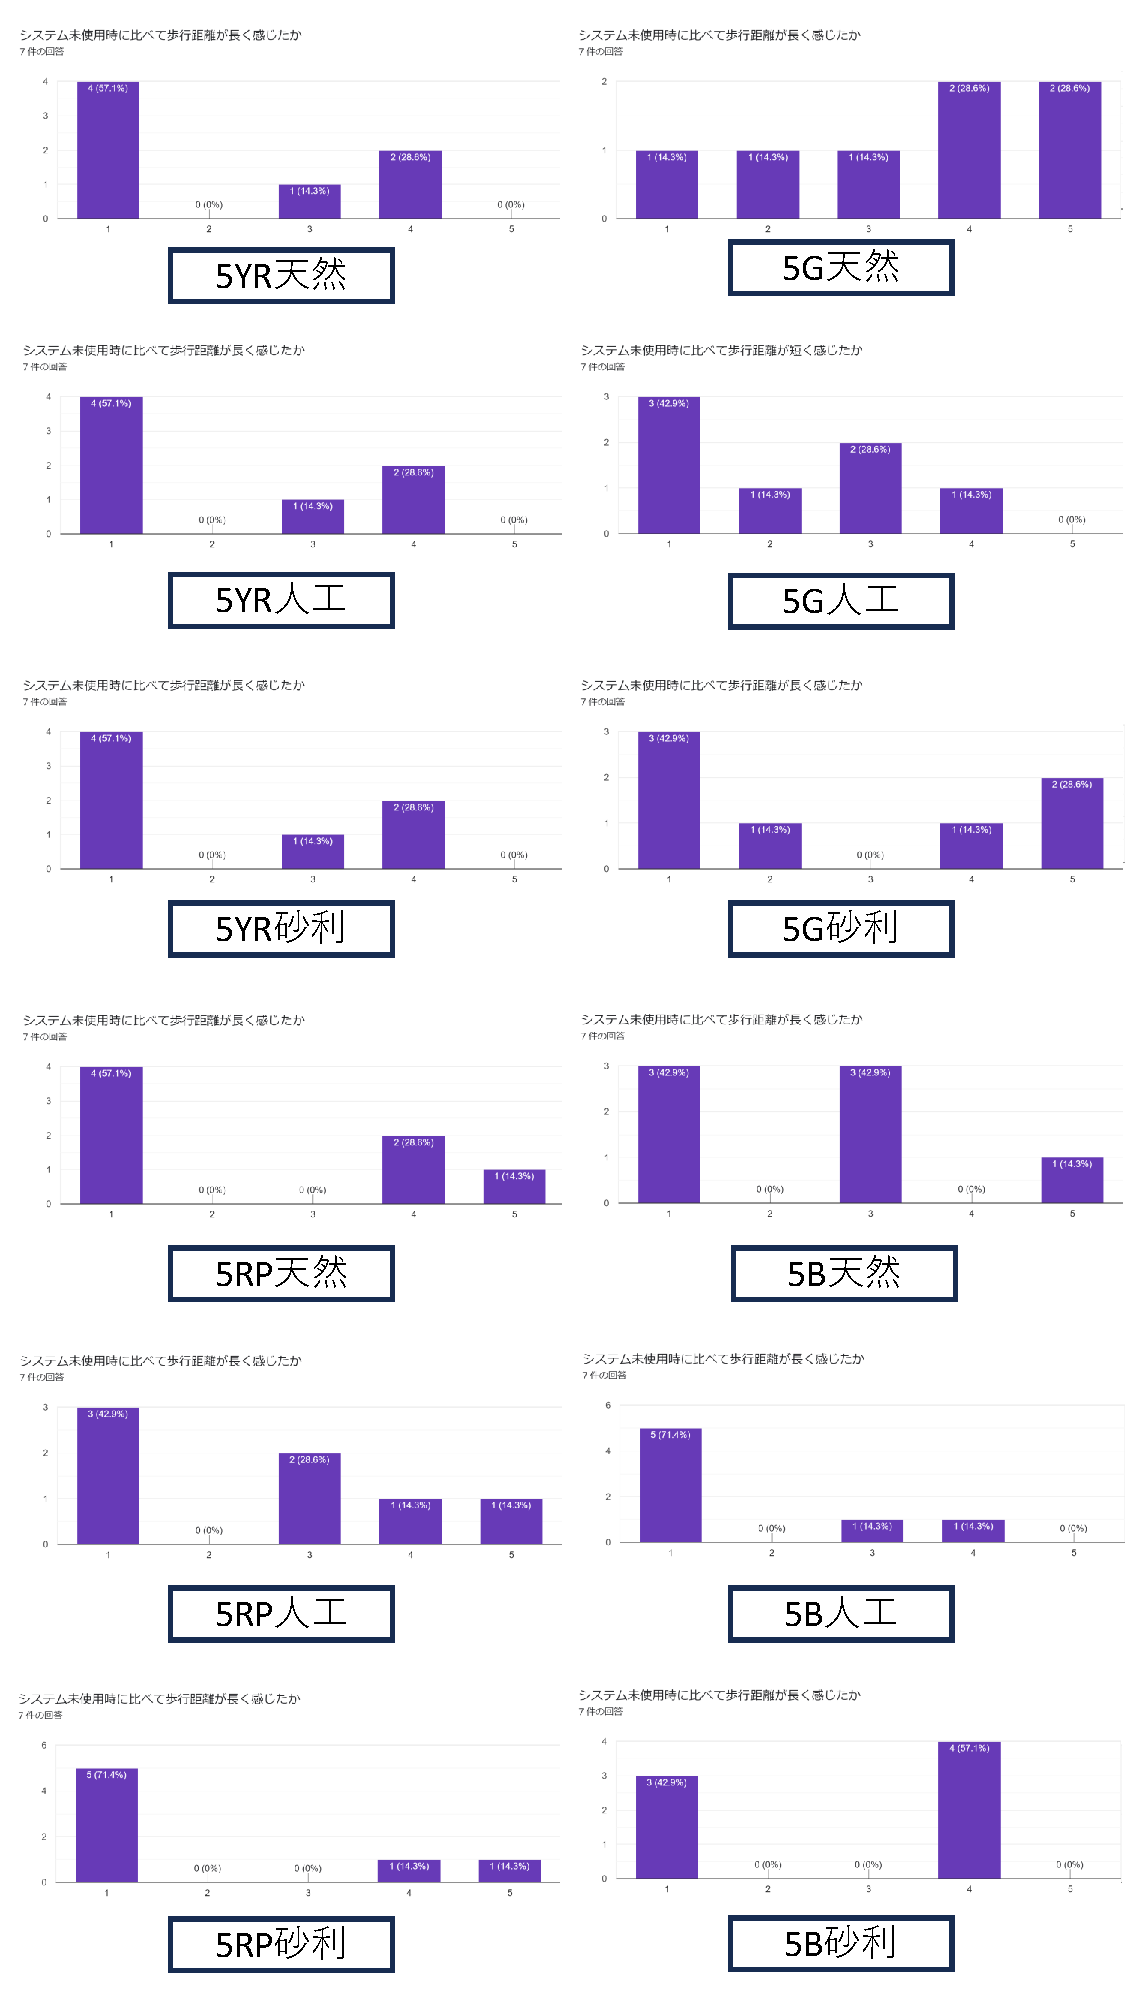
\includegraphics[width=0.8\linewidth]{fig/(前)longer.pdf}
    }
    \caption{バーチャル床が前から迫ってくることで歩行距離が長く感じたかのアンケート結果}
    \label{fig:f4}
\end{figure}
\begin{figure}[H]
    \centering
    \fbox{
        \includegraphics[width=0.8\linewidth]{fig/(後)faster.pdf}
    }
    \caption{バーチャル床が後ろから追い越してくることで早い速度感を得たかのアンケート結果}
    \label{fig:b1}
\end{figure}
\begin{figure}[H]
    \centering
    \fbox{
        \includegraphics[width=0.8\linewidth]{fig/(後)slower.pdf}
    }
    \caption{バーチャル床が後ろから追い越してくることで遅い速度感を得たかのアンケート結果}
    \label{fig:b2}
\end{figure}
\begin{figure}[H]
    \centering
    \fbox{
        \includegraphics[width=0.8\linewidth]{fig/(後)shoater.pdf}
    }
    \caption{バーチャル床が後ろから追い越してくることで歩行距離が短く感じたかのアンケート結果}
    \label{fig:b3}
\end{figure}
\begin{figure}[H]
    \centering
    \fbox{
        \includegraphics[width=0.8\linewidth]{fig/(後)longer.pdf}
    }
    \caption{バーチャル床が後ろから追い越してくることで歩行距離が長く感じたかのアンケート結果}
    \label{fig:b4}
\end{figure}

\begin{figure}[H]
    \centering
    \fbox{
        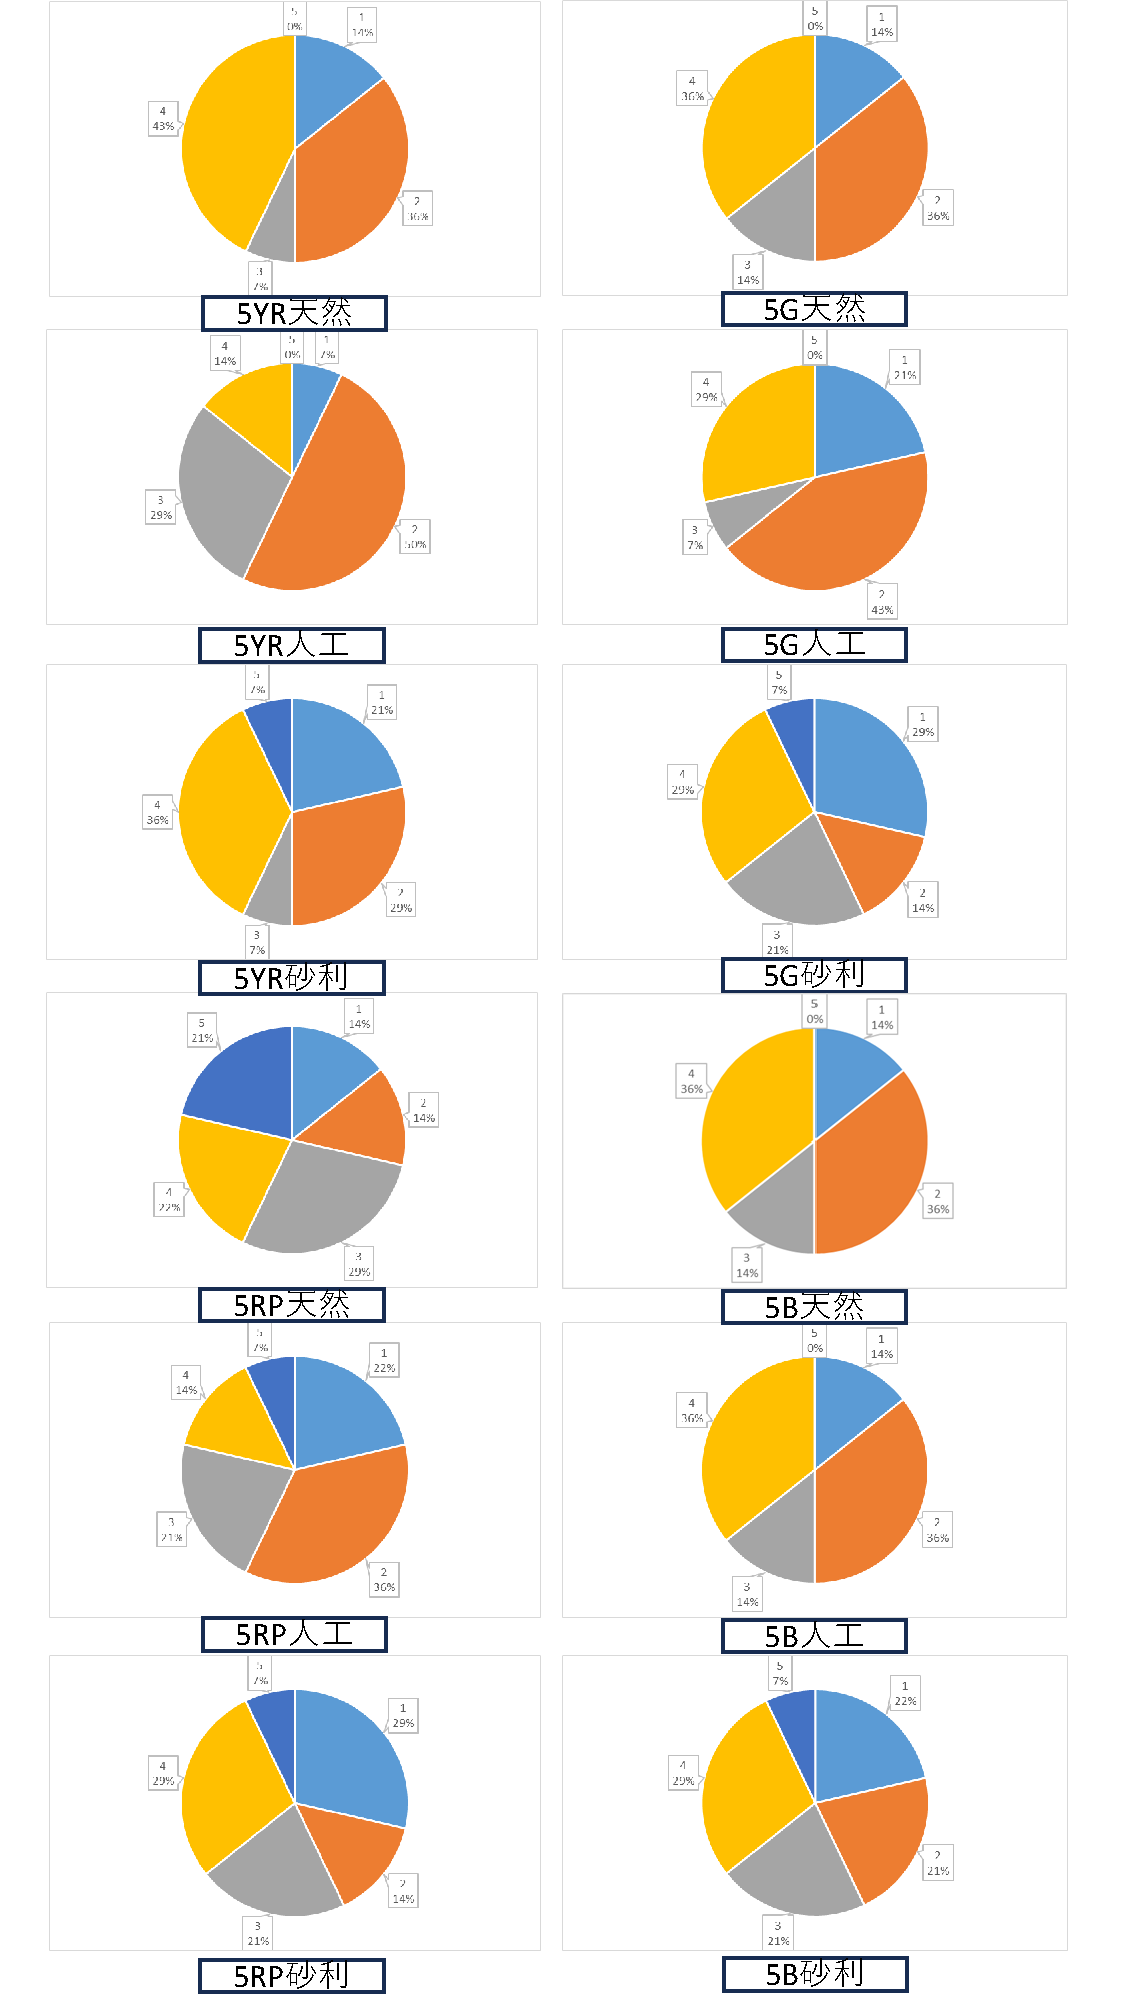
\includegraphics[width=0.8\linewidth]{fig/similar.pdf}
    }
    \caption{バーチャル床は本物の床が動いているように見えたかのアンケート結果}
    \label{fig:simi}
\end{figure}

\begin{figure}[H]
    \centering
    \fbox{
        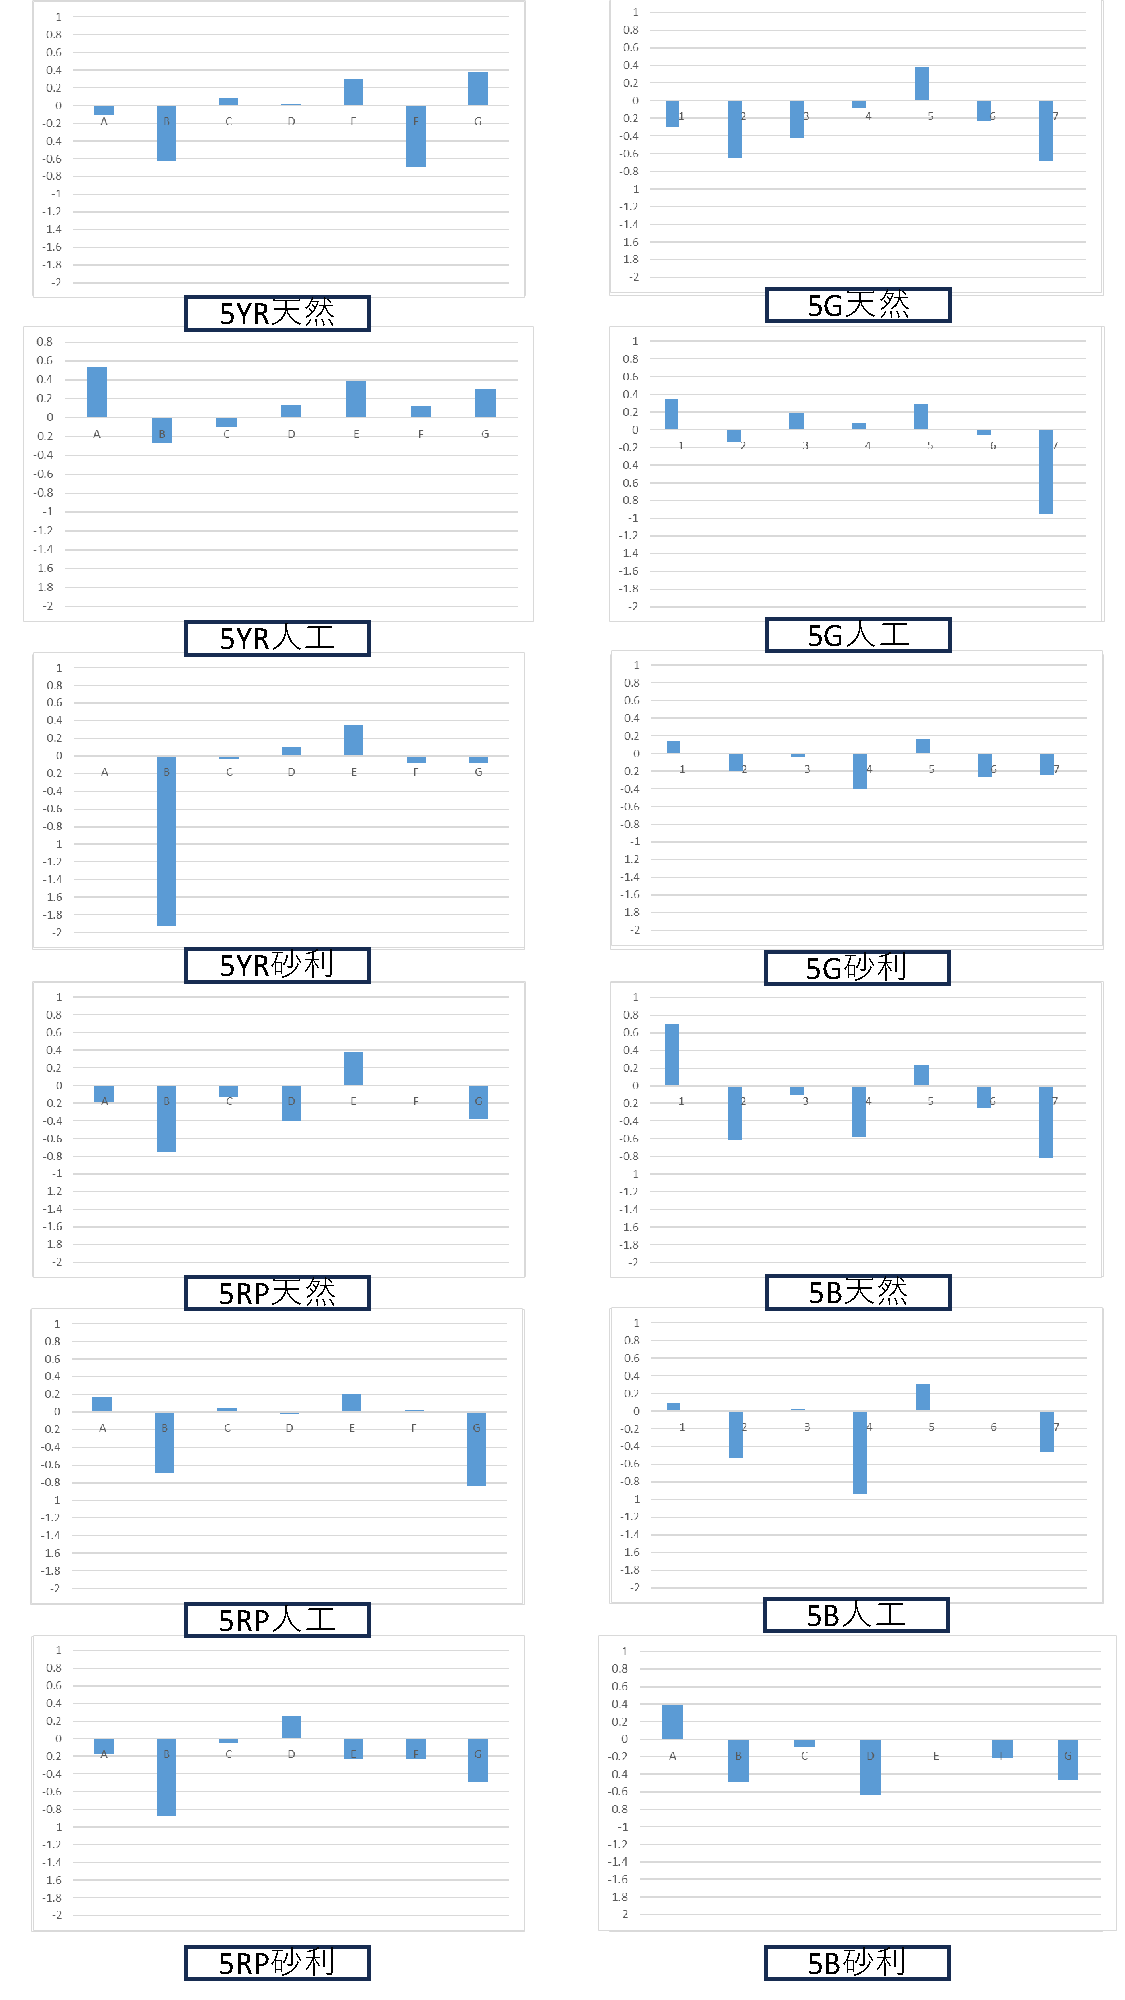
\includegraphics[width=0.8\linewidth]{fig/(前)halftime.pdf}
    }
    \caption{システム未使用時とシステム(前から迫ってくる)使用時の中間地点までの時間差一覧}
    \label{fig:maehalf}
\end{figure}
\begin{figure}[H]
    \centering
    \fbox{
        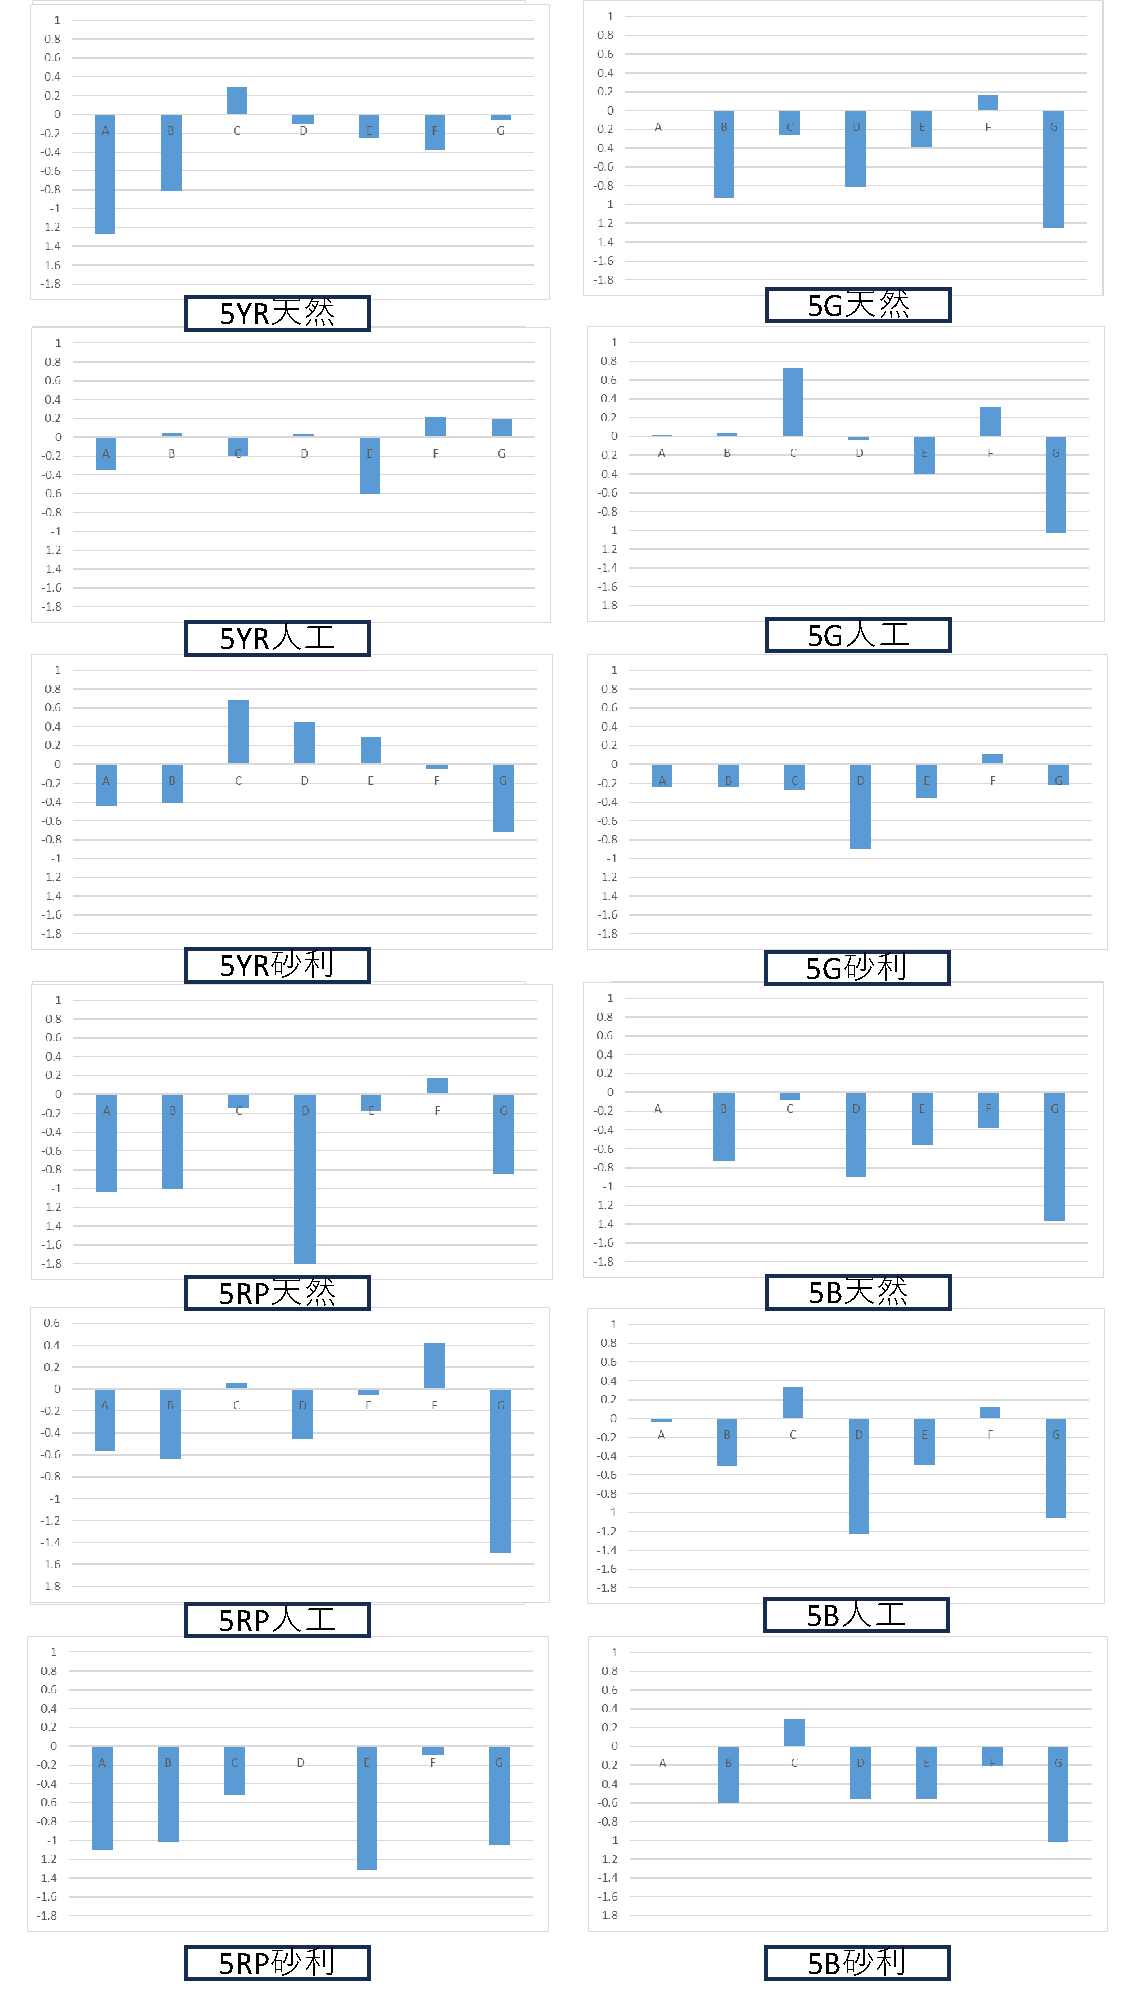
\includegraphics[width=0.8\linewidth]{fig/(前)time.pdf}
    }
    \caption{システム未使用時とシステム(前から迫ってくる)使用時のゴールまでの時間差一覧}
    \label{fig:maetime}
\end{figure}
\begin{figure}[H]
    \centering
    \fbox{
        \includegraphics[width=0.8\linewidth]{fig/(後)halftime.pdf}
    }
    \caption{システム未使用時とシステム(後ろから追い越してくる)使用時の中間地点までの時間差一覧}
    \label{fig:usirohalf}
\end{figure}
\begin{figure}[H]
    \centering
    \fbox{
        \includegraphics[width=0.8\linewidth]{fig/(後)time.pdf}
    }
    \caption{システム未使用時とシステム(後ろから追い越してくる)使用時のゴールまでの時間差一覧}
    \label{fig:usirotime}
\end{figure}	% 付録



\end{document}
